\chapter{โมเดลเชิงเส้น}
\label{chapter: Linear Models}

\begin{verse}
``If I have seen further, it is by standing upon the shoulders of giants.''\\
---Sir Isaac Newton
\end{verse}

\begin{verse}
``ถ้าผมมองเห็นได้ยาวไกล มันก็ได้มาด้วยการยืนบนไหล่ของยักษ์''\\
---เซอร์ ไอแซค นิวตัน
\end{verse}


บท~\ref{chapter: background} อภิปรายการใช้ฟังชั่นพหุนามในการทำนายค่าเอาต์พุต.
การสร้างโมเดล เพื่อทำนายค่าของเอาต์พุตโดยที่เอาต์พุตเป็นค่าต่อเนื่อง จะเรียกว่า \textit{การหาค่าถดถอย} (Regression).
\index{regression}
\index{การหาค่าถดถอย}
%
\textit{โมเดลพหุนาม}เป็นหนึ่งในตัวอย่างของกลุ่มโมเดลที่นิยมใช้ในการหาค่าถดถอย 
เรียกว่า \textit{กลุ่มโมเดลหาค่าถดถอยเชิงเส้น} (Linear Regression Model) หรือสั้นๆว่า \textit{โมเดลเชิงเส้น}.
คุณสมบัติที่สำคัญของ\textit{โมเดลเชิงเส้น} ก็คือ 
ค่าของเอาต์พุตของโมเดลจะมีความสัมพันธ์เชิงเส้นกับค่าพารามิเตอร์ของโมเดล.
เช่นในกรณีของฟังชั่นพหุนาม ค่าเอาต์พุต $y$ มีความสัมพันธ์เชิงเส้นกับ $\mathbf{w}$ ใน $y = w_0 + w_1 x + w_2 x^2 + \cdots + w_M x^M$ เมื่อ $x$ คืออินพุต.
สังเกตุว่า โมเดลเชิงเส้นมีเอาต์พุตที่มีความสัมพันธ์เชิงเส้นกับพารามิเตอร์ แต่ไม่จำเป็นว่าเอาต์พุตต้องมีความสัมพันธ์เชิงเส้นกับอินพุต.
และ เทอมต่างๆที่คูณอยู่กับพารามิเตอร์แต่ละตัว จะเรียกว่า \textit{เบซิสฟังชั่น} (ฺBasis Functions) 
เช่นในกรณีฟังชั่นพหุนาม ก็คือ $1, x, x^2, \ldots, x^M$.
นั่นคือ กำหนดให้ \textit{เบซิสฟังชั่น} $\phi_m(x) = x^m$ เมื่อ $m = 0, 1, \ldots, M$.

\section{การหาค่าถดถอยเชิงเส้น}
\label{section: Linear Regression Model}
\index{linear regression model}
\index{โมเดลการหาค่าถดถอยเชิงเส้น}

ในกรณีที่อินพุตเป็นตัวแปรเดี่ยว (Scalar Variable, $x \in \mathbb{R}$) 
ฟังชั่นพหุนามเป็นโมเดลเชิงเส้นที่สามารถใช้ทำการหาค่าถดถอยได้.
แต่หากต้องการทำนายค่าเอาต์พุตจากอินพุต โดยที่อินพุตเป็น\textit{ตัวแปรหลายมิติ} (Multi-Dimensional Variable, $\mathbf{x} \in \mathbb{R}^D, D > 1$) เช่น ตัวอย่างการทำนายปริมาณคาร์บอนไดออกไซด์ในอากาศ ในฤดูการเก็บเกี่ยวอ้อย%
\footnote{ถึงแม้การเป็นการสร้างมลภาวะอย่างมาก รวมถึงความเสียหายอื่น เช่น สายไฟฟ้าในบริเวณใกล้เคียง  ทัศนวิสัย ความเสี่ยงที่ไม่สามารถควบคุมไฟได้, การเผาอ้อยเพื่อเก็บเกี่ยวก็ยังเป็นปัญหาด้านความปลอดภัย สิ่งแวดล้อม และสร้างปัญหาสุขภาพกับประเทศไทยอยู่.} จาก อุณหภูมิ ความเร็วลม ความชื้น และขนาดพื้นที่ของไร่อ้อยที่มีการเผาก่อนเก็บเกี่ยวในบริเวณใกล้เคียง.
กรณีนี้ อินพุตมี $4$ มิติ.
นั่นคือ $\mathbf{x} = [x_1, x_2, x_3, x_4]^T$ สำหรับ อุณหภูมิ ความเร็วลม ความชื้น และขนาดพื้นที่ ตามลำดับ.

สำหรับกรณีที่อินพุตเป็นตัวแปร $D$ มิติ 
โมเดลเชิงเส้นแบบที่ง่ายที่สุด ก็คือ\textit{โมเดลการหาค่าถดถอยเชิงเส้น} (Linear Regression),
\begin{eqnarray}
   y(\mathbf{x}, \mathbf{w}) = w_0 + w_1 x_1 + \ldots + w_D x_D 
\label{eq: linear regression}
\end{eqnarray}
เมื่อ $\mathbf{x} = [x_1, x_2, \ldots, x_D]^T$.

แทนที่จะใช้อินพุตโดยตรง เบซิสฟังชั่นสามารถนำมาใช้เพื่อเพิ่มความสามารถของโมเดลได้
ดังสมการที่เป็นการรวมเชิงเส้นของเบซิสฟังชั่น,
\begin{eqnarray}
   y(\mathbf{x}, \mathbf{y}) = w_0 + \sum_{j=1}^{M-1} w_j \phi_j(\mathbf{x})
\label{eq: linear regression model}
\end{eqnarray}
เมื่อ $\phi_j(\mathbf{x})$ คือ เบซิสฟังชั่น.
สมการนี้ใช้ค่าดัชนี $j$ วิ่งไปถึงค่าสูงสุดที่ $M-1$ เพื่อความสะดวกที่จะได้มีจำนวนพารามิเตอร์ทั้งหมดเป็น $M$ ตัว.
พารามิเตอร์ $w_0$ คือ ค่าออฟเซต (Offset) หรือ บางครั้งเรียกว่า ค่าไบอัส (Bias).

เพื่อความสะดวก นิยาม $\phi_0(\mathbf{x}) = 1$ ซึ่งทำให้
\begin{eqnarray}
   y(\mathbf{x}, \mathbf{y}) = \sum_{j=0}^{M-1} w_j \phi_j(\mathbf{x}) = \mathbf{w}^T \bm{\phi}(\mathbf{x})
\label{eq: linear regression model short}
\end{eqnarray}
เมื่อ $\mathbf{w} = [w_0, \ldots, w_{M-1}]^T$ และ $\bm{\phi}(\mathbf{x})$ แทน $[\phi_0(\mathbf{x}), \ldots, \phi_{M-1}(\mathbf{x})]^T$.

เราอาจมองเบซิสฟังชั่น $\bm{\phi}(\mathbf{x})$ ว่าเป็น \textit{ลักษณะสำคัญ} (Features) ของอินพุตได้.
ถ้าหากเลือกเบซิสฟังชั่นเป็น\textit{ฟังชั่นไม่เป็นเชิงเส้น} (Non-Linear Function) ของอินพุต เราก็จะมีโมเดลที่เอาต์พุตมีความสัมพันธ์\textit{ไม่เป็นเชิงเส้น}กับอินพุตได้ ในขณะที่เอาต์พุตมีความสัมพันธ์เชิงเส้นกับพารามิเตอร์อยู่.
การที่เอาต์พุตมีความสัมพันธ์เชิงเส้นกับพารามิเตอร์ จะทำให้การวิเคราะห์และการฝึกโมเดลทำได้ง่าย ดังที่จะได้เห็นต่อไป (หัวข้อ~\ref{section: linear maximum likelihood})

ตามที่กล่าวไปข้างต้น ฟังชั่นพหุนามเป็นกรณีที่ $\phi_j(x) = x^j$.
การใช้เบซิสฟังชั่นแบบนี้ จะทำให้โมเดลมีคุณสมบัติเป็น\textit{ฟังชั่นทั่วถึง} (Global Function) กับอินพุต. 
นั่นคือ ถ้าอินพุตค่าช่วงหนึ่งเปลี่ยนแปลง ก็จะมีผลกับเบซิสฟังชั่นทุกๆตัว.

หากไม่ต้องการคุณสมบัติ\textit{ฟังชั่นทั่วถึง} %เราอาจจะแบ่งเบซิสฟังชั่นให้การตอบสนองไม่เท่ากันต่ออินพุตจากแต่ละส่วนของ\textit{ปริภูมิอินพุต} (Input Space).
ก็อาจเลือกใช้เบซิสฟังชั่นที่มีลักษณะเป็น\textit{ฟังชั่นท้องถิ่น}
เช่น การใช้\textit{เกาส์เชี่ยนเบซิสฟังชั่น} (Gaussian Basis Function).
%
\textit{เกาส์เชี่ยนเบซิสฟังชั่น}นิยามได้ดังนี้
\begin{eqnarray}
   \phi_j(x) = \exp \left( -\frac{(x - \mu_j)^2}{2 s^2} \right)
\label{eq: gaussian basis function}
\end{eqnarray}
เมื่อ $\mu_j$ เป็นโมเดลพารามิเตอร์ 
ซึ่ง $\mu_j$ ทำหน้าที่เสมือนตำแหน่งใน\textit{ปริภูมิอินพุต}ที่ทำให้อินพุตมีผลต่อเบซิสฟังชั่นมากที่สุด.
นั่นคือ ยิ่่ง $x$ มีค่าใกล้ $\mu_j$ เท่าไร $\phi_j$ ก็จะตอบสนองได้ดีเท่านั้น 
และ $s$ เป็นโมเดลพารามิเตอร์ทำหน้าที่เหมือนสเกลปรับลดขยายผลการตอบสนอง $\phi_j$.
รูป~\ref{fig: gaussian basis function} แสดงการตอบสนองของเบซิสฟังชั่นต่ออินพุต ที่ $\mu_j$ และ $s$ ต่างๆ.

%
\begin{figure}
\begin{center}
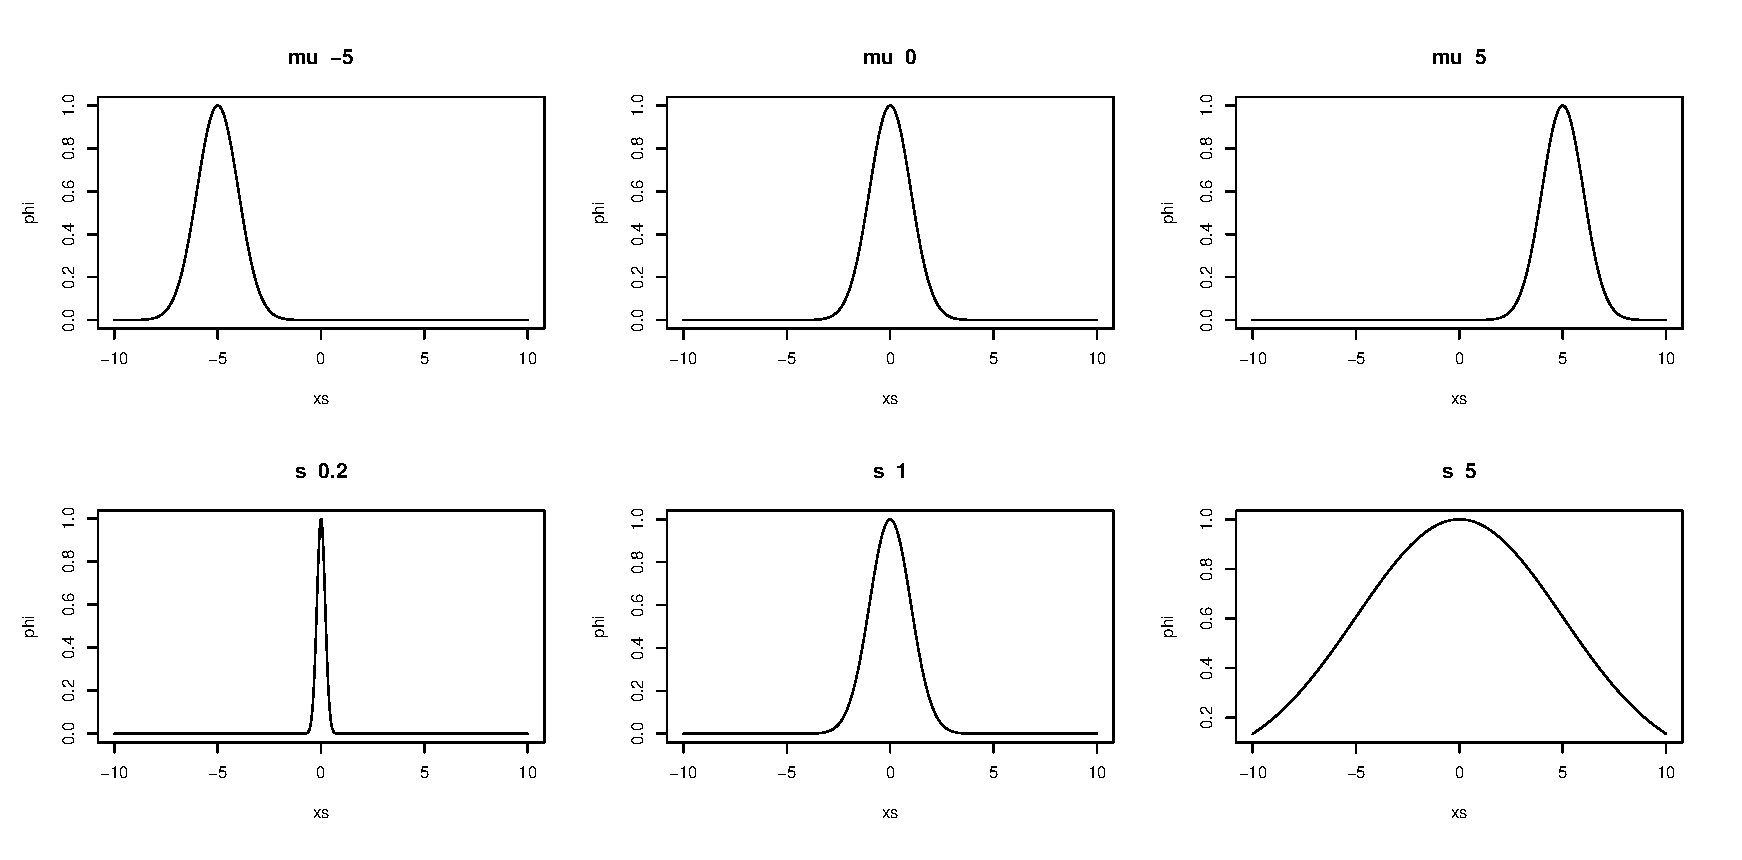
\includegraphics[height=2in]{02Background/gaussianBasis.eps}
\end{center}
\caption{เกาส์เชี่ยนเบซิสฟังชั่นที่ค่าสเกล $s$ และตำแหน่ง $\mu_j$ ต่างๆ}
\label{fig: gaussian basis function}
\end{figure}
%

หรือ ผู้ใช้อาจเลือกซิกมอยด์เบซิสฟังชั่น (Sigmoid Basis Function),
\begin{eqnarray}
   \phi_j(x) = \sigma \left( \frac{x - \mu_j}{s} \right)
\label{eq: sigmoid basis function}
\end{eqnarray}
เมื่อ $\sigma(a)$ คือซิกมอยด์ฟังชั่น (Sigmoid Function)
หรืออีกชื่อคือ โลจิสติกฟังชั่น (Logistic Function),
\begin{eqnarray}
   \sigma(a) = \frac{1}{1+\exp(-a)}.
\end{eqnarray}
รูป~\ref{fig: sigmoid basis function} แสดงการตอบสนองของซิกมอยด์เบซิสฟังชั่นต่ออินพุต ที่ $\mu_j$ และ $s$ ต่างๆ.
สังเกตุ ค่า $\mu_j$ มีผลต่อตำแหน่งของรูปทรง.
ส่วน $s$ ความคุมสเกลหรือการยืดหดในแนวนอนของรูปทรง (แต่ยังเป็นทรงตัว `S' เหมือนเดิม).

%
\begin{figure}
\begin{center}
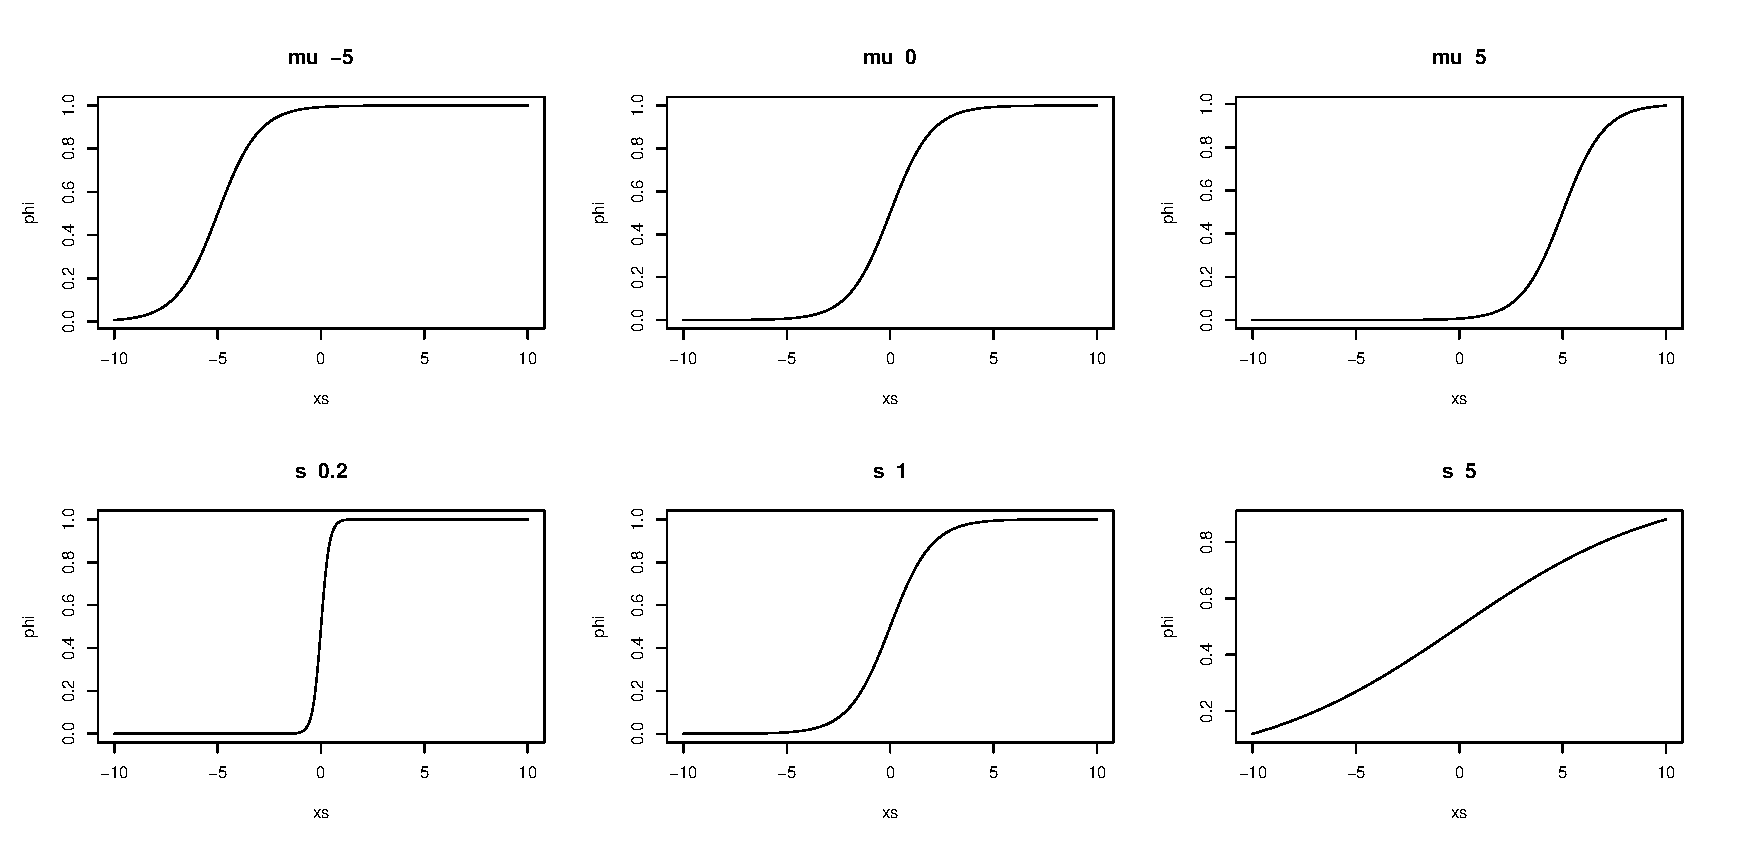
\includegraphics[height=2in]{02Background/sigmoidBasis.eps}
\end{center}
\caption{ซิกมอยด์เบซิสฟังชั่นที่ค่าสเกล $s$ และตำแหน่ง $\mu_j$ ต่างๆ}
\label{fig: sigmoid basis function}
\end{figure}
%

%Fourier basis ก็เป็น เบซิสฟังชั่นที่นิยม อีกชนิด, เหมาะสำหรับโมเดล ระบบที่มีลักษณะเป็นคาบ.


\subsection{วิธีจัดแล้วพอดีที่สุด}
\label{section: linear maximum likelihood}

หากมองว่า ความสัมพันธ์ระหว่างเอาต์พุต $t$ กับอินพุต $\mathbf{x}$ 
คือผลรวมจาก\textit{ฟังชั่นเชิงกำหนด}กับสัญญาณรบกวน,
\begin{eqnarray}
   t = y(\mathbf{x}, \mathbf{w}) + \epsilon
\label{eq: linear deterministic and stochastic parts}
\end{eqnarray} 
เมื่อ $y(\mathbf{x}, \mathbf{w})$ เป็น\textit{ฟังชั่นเชิงกำหนด} (Deterministic Model) มีพารามิเตอร์ $\mathbf{w}$, กรณีนี้เราจะใช้โมเดลเชิงเส้น (สมการ~\ref{eq: linear regression model short}).
และ $\epsilon$ เป็นสัญญาณรบกวนแบบเกาส์เชี่ยนที่มีค่าเฉลี่ยเป็น $0$.
ดังนั้นสามารถเขียนความน่าจะเป็นแบบมีเงื่อนไข $p(t|\mathbf{x})$ ได้ว่า
\begin{eqnarray}
   p(t|\mathbf{x}, \mathbf{w}, \beta) 
   &=& \mathcal{N}(t|y(\mathbf{x}, \mathbf{w}), \beta^{-1})
\label{eq: linear gaussian model}
\end{eqnarray}
โดยตัวแปร $\mathbf{w}$ และ $\beta$ เป็นพารามิเตอร์ 
และ $\mathcal{N}(t|y(\mathbf{x}, \mathbf{w}), \beta^{-1})$ แทนการกระจายแบบเกาส์เชี่ยน
ซึ่งนั่นคือ
\begin{eqnarray}
  \mathcal{N}(\mathbf{z}|\mathbf{\mu}, \sigma^2)
  &=& \frac{1}{(2 \pi \sigma^2)^{D/2}}
  \exp \left\{ -\frac{1}{2 \sigma^2} (\mathbf{z} - \mathbf{\mu})^2 \right\}
\nonumber 
\end{eqnarray}
สำหรับ $\mathbf{z} \in \mathbb{R}^D$.
%$\mathcal{N}(t|y(\mathbf{x}, \mathbf{w}), \beta^{-1})$ แทนการกระจายแบบเกาส์เชี่ยน ที่มีค่าเฉลี่ย $\mu = y(\mathbf{x}, \mathbf{w}) = \mathbf{w}^T \mathbf{x}$ และค่าแปรปรวน $\sigma^2 = \beta^{-1}$.
%(ดูสมการ~\ref{eq: one-D gaussian distribution}, หัวข้อ~\ref{section: Probability}). 

ถ้ามีข้อมูล $\mathcal{D}$ ซึ่งประกอบด้วยอินพุต $\mathbf{X} = \{ \mathbf{x}_1, \mathbf{x}_2, \ldots, \mathbf{x}_N \}$ และเอาต์พุต $\mathbf{T} = \{t_1, t_2, \ldots, t_N\}$ ตามลำดับ.
โดยมีสมมติฐานว่า แต่ละจุดข้อมูลเป็น i.i.d. (independent and identically distributed) แบบในสมการ~\ref{eq: linear gaussian model}, \textit{ฟังก์ชันควรจะเป็น}ของข้อมูลชุดนี้ คือ 
%
\begin{eqnarray}
   p(\mathbf{T} | \mathbf{X}, \mathbf{w}, \beta) 
   &=& \prod_{n=1}^N \mathcal{N}( t_n | y(\mathbf{x}_n , \mathbf{w}), \beta^{-1})
\label{eq: linear likelihood} \\
   &=& \prod_{n=1}^N \mathcal{N}( t_n | \mathbf{w}^T \bm{\phi} ( \mathbf{x}_n ), \beta^{-1})
\label{eq: linear likelihood linear model}
\end{eqnarray}

ตอนนี้ก็สามารถใช้\textit{วิธีจัดแล้วพอดีที่สุด} (Maximum Likelihood) เพื่อหาค่าพารามิเตอร์ $\mathbf{w}$ และ $\beta$ ที่ทำให้ได้\textit{ฟังก์ชันควรจะเป็นมีค่ามากที่สุด}.

ในทางปฏิบัติค่าความน่าจะเป็นของข้อมูลแต่ละจุดมีค่าน้อย
และเมื่อทำการคูณความน่าจะเป็นของทุกๆจุดเข้าด้วยกันอาจทำให้เกิดปัญหาเชิงเลข
ที่ไม่สามารถแทนค่า\textit{ฟังก์ชันควรจะเป็น}ค่าน้อยๆได้
วิธีแก้ปัญหาคือใช้ลอการิทึ่มเข้ามาช่วย โดยคุณสมบัติของลอการิทึ่มจะช่วยแก้ปัญหาการคำนวณเชิงเลขในทางปฏิบัติได้
และไม่ได้ทำให้จุดประสงค์ที่ต้องการเปลี่ยนไป
ดังนั้นเมื่อใส่ลอการิทึ่มเข้าไปกับสมการ~\ref{eq: linear likelihood} จะได้
\begin{eqnarray}
   \ln p(\mathbf{T} | \mathbf{X}, \mathbf{w}, \beta)
   &=& \sum_{n=1}^N \ln \mathcal{N}( t_n | y(\mathbf{x}_n , \mathbf{w}), \beta^{-1})
\nonumber \\
   &=& \frac{N}{2} \ln \beta - \frac{N}{2} \ln (2 \pi) - \beta E_{\mathcal{D}}(\mathbf{w})
\label{eq: linear log likelihood}   
\end{eqnarray}
เมื่อ
\begin{eqnarray}
   E_{\mathcal{D}}(\mathbf{w}) &=& \frac{1}{2} \sum_{n=1}^N \{ t_n - \mathbf{w}^T \bm{\phi}(\mathbf{x}_n) \}^2.
\label{eq: linear Error}
\end{eqnarray}

แล้วเกรเดียนต์ของ\textit{ลอการิทึ่มฟังก์ชันควรจะเป็น} เมื่อเทียบกับ $\mathbf{w}$ ก็สามารถหาได้ว่า
\begin{eqnarray}
   \nabla \ln p(\mathbf{T} | \mathbf{w}, \beta) 
   = \beta \cdot \sum_{n=1}^N \left\{ t_n - \mathbf{w}^T \bm{\phi} (\mathbf{x}_n) \right\} \bm{\phi}(\mathbf{x}_n)^T.
\label{eq: linear gradient log likelihood}
\end{eqnarray}

จากเงื่อนไขจำเป็นอันดับแรก (ดูหัวข้อ~\ref{sec: opt FONC}) 
กำหนดให้ $\nabla \ln p(\mathbf{T} | \mathbf{w}, \beta) = 0$ และจัดรูปใหม่ จะได้,
\begin{eqnarray}
   \mathbf{0} = \sum_{n=1}^N t_n \bm{\phi}(\mathbf{x}_n)^T - \mathbf{w}^T \cdot \sum_{n=1}^N  \bm{\phi} (\mathbf{x}_n)  \bm{\phi}(\mathbf{x}_n)^T.
\label{eq: linear gradient log likelihood 0}
\end{eqnarray}
ซึ่งคือได้
\begin{eqnarray}
   \mathbf{w}_{ML} &=& (\Phi^T \Phi)^{-1} \Phi^T \mathbf{T}
\label{eq: linear W} \\
   \Phi &=& \begin{bmatrix}
   \phi_0(\mathbf{x}_1) & \phi_1(\mathbf{x}_1) & \phi_2(\mathbf{x}_1) & \ldots & \phi_{M-1}(\mathbf{x}_1) \\
   \phi_0(\mathbf{x}_2) & \phi_1(\mathbf{x}_2) & \phi_2(\mathbf{x}_2) & \ldots & \phi_{M-1}(\mathbf{x}_2) \\
   \phi_0(\mathbf{x}_3) & \phi_1(\mathbf{x}_3) & \phi_2(\mathbf{x}_3) & \ldots & \phi_{M-1}(\mathbf{x}_3) \\
   \vdots & \vdots & \vdots & \ddots & \vdots \\
   \phi_0(\mathbf{x}_N) & \phi_1(\mathbf{x}_N) & \phi_2(\mathbf{x}_N) & \ldots & \phi_{M-1}(\mathbf{x}_N)   
   \end{bmatrix}.
\label{eq: linear Moore-Penrose pseudo-inverse}
\end{eqnarray}

ลักษณะเดียวกัน เมื่อหาค่าของ $\beta$ ที่ทำให้สมการ~\ref{eq: linear log likelihood} มีค่ามากที่สุด ก็จะได้
\begin{eqnarray}
   \frac{1}{\beta_{ML}} = \frac{1}{N} \sum_{n=1}^N \left\{ t_n - \mathbf{w}_{ML}^T \bm{\phi}(\mathbf{x}_n) \right\}^2.
\label{eq: linear beta}   
\end{eqnarray}
สังเกตุ สมการ~\ref{eq: linear beta} คือค่าแปรปรวนของเอาต์พุต $t_n$ เทียบกับค่าเฉลี่ยจากโมเดลเชิงเส้น.

\subsection{การเรียนรู้โดยลำดับ}
\label{section: sequential learning}

การหาค่าพารามิเตอร์ด้วยสมการ~\ref{eq: linear W} และ~\ref{eq: linear beta} 
จะใช้ข้อมูล $\mathcal{D}$ ทั้งหมดในการฝึกทีเดียว.
ลักษณะการฝึกแบบใช้ข้อมูลทั้งหมดทีเดียวแบบนี้จะเรียกว่า เป็น\textit{การฝึกแบบกลุ่ม} 
หรือ\textit{การเรียนรู้แบบกลุ่ม} (Batch Learning).
\index{batch learning} \index{การฝึกแบบกลุ่ม} \index{การเรียนรู้แบบกลุ่ม}

แต่ถ้าข้อมูลมีขนาดใหญ่มากๆ การเรียนรู้แบบกลุ่มนี้อาจจะมีปัญหากับการทำการคำนวณได้ 
เพราะเมตริกซ์ $\Phi$ (สมการ~\ref{eq: linear Moore-Penrose pseudo-inverse}) จะมีขนาดใหญ่มาก.
นอกจากนั้น หากมีข้อมูลใหม่เพิ่มขึ้นมา เราจะต้องทำการรวมกับข้อมูลเก่า และฝึกกับข้อมูลทั้งหมดทีเดียว.
วิธีที่มีประสิทธิภาพกว่า ในกรณีที่มีข้อมูลขนาดใหญ่มากๆ หรือกรณีที่มีข้อมูลมาเพิ่ม คือ การใช้\textit{การฝึกโดยลำดับ} หรือ\textit{การเรียนรู้โดยลำดับ} (Sequential Learning หรือ Online Learning).

\textit{การเรียนรู้โดยลำดับ}จะใช้จุดข้อมูลทีละจุดในการปรับค่าพารามิเตอร์.
การเรียนรู้โดยลำดับยังเหมาะกับ\textit{แอฟพลิเคชั่นตามเวลาจริง} (Real-Time Applications) ที่ข้อมูลใหม่จะเข้ามาเรื่อยๆ และระหว่างนั้นก็สามารถจะใช้ค่าพารามิเตอร์ล่าสุดในการทำงานได้ โดยไม่ต้องรอให้ได้ข้อมูลมาครบ.

วิธีลงเกรเดียนต์ (หัวข้อ~\ref{section: Optimization}) สามารถนำมาใช้เพื่อช่วยในกระบวนการเรียนรู้โดยลำดับ ดังนี้
\begin{eqnarray}
   \mathbf{w}^{(k+1)} &=& \mathbf{w}^{(k)} - \alpha \cdot \nabla \{- \ln p(\mathbf{T}|\mathbf{X}, \mathbf{w}, \beta) \}
\label{eq: linear w online}
\end{eqnarray}
เมื่อ $k$ คือดัชนีแทนครั้งที่คำนวณ, $\alpha$ คือ\textit{ค่าขนาดก้าว} 
(หรือสำหรับการเรียนรู้ของเครื่อง ค่านี้มักถูกเรียกว่า \textit{อัตราการเรียนรู้}, Learning Rate),
$\mathbf{X}$ และ $\mathbf{T}$ คือข้อมูลที่จะใช้ในการคำนวณครั้งที่ $k$.

สังเกตุ วิธีลงเกรเดียนต์ออกแบบมาสำหรับ\textit{ปัญหาการหาตัวทำน้อยที่สุด} 
แต่\textit{วิธีจัดแล้วพอดีที่สุด}เป็น\textit{ปัญหาการหาตัวทำมากที่สุด}
ฉะนั้นฟังชั่นเป้าหมายจึงใช้ $- \ln p(\mathbf{T}|\mathbf{X}, \mathbf{w}, \beta)$ 
โดยเครื่องหมายลบใช้เพื่อแปลงปัญหาการหาตัวทำมากที่สุดมาเป็นปัญหาการหาตัวทำน้อยที่สุด (ดูหัวข้อ~\ref{section: Optimization} เพิ่มเติม)


สำหรับโมเดลเชิงเส้น (ดูสมการ~\ref{eq: linear gradient log likelihood} เปรียบเทียบ),
%~\ref{eq: linear log likelihood} และ \ref{eq: linear Error}
จะได้สมการปรับค่าพารามิเตอร์ว่า
\begin{eqnarray}
   \mathbf{w}^{(k+1)} &=& \mathbf{w}^{(k)} + \alpha \cdot \left(  t_n - \mathbf{w}^{(k) T} \bm{\phi}(\mathbf{x}_n) \right) \bm{\phi}(\mathbf{x}_n)
\label{eq: linear w online linear model}
\end{eqnarray}
โดย เช่นเดียวกับวิธีลงเกรเดียนต์ ค่าอัตราการเรียนรู้จะต้องเลือกให้เหมาะสม 
อาทิ ไม่ใหญ่เกินไป เพื่อให้อัลกอริทึ่ม\textit{ลู่เข้า} 
หรือ ไม่เล็กเกินไป เพื่อจะได้ไม่ต้องทำการคำนวณหลายรอบมากเกินไป. %ก่อนที่จะได้ค่า $\mathbf{w}$ ที่ดี.

\section{เรกูลาไรเซชั่น}
\label{sec: regularization}
\index{regularization}
\index{เรกูลาไรเซชั่น}

บทที่~\ref{chapter: background} อภิปรายเรื่อง\textit{เรกูลาไรเซชั่น} (Regularization) ได้บ้าง. ซึ่ง\textit{เรกูลาไรเซชั่น} คือการควบคุมค่าของพารามิเตอร์ไม่ให้ใหญ่เกินไป เพื่อลดปัญหา\textit{โอเวอร์ฟิตติ้ง} (Overfitting)
โดยใช้กลไกของ\textit{พีนอตี้}ที่เพิ่มเข้าไปในฟังชั่นเป้าหมาย ได้แก่ การนิยาม \textit{ฟังชั่นค่าผิดพลาดรวม} (Total Error Function) เป็น
\[
  E_{total}(\mathbf{w}) = E_D(\mathbf{w}) + \lambda E_W(\mathbf{w})
\]
โดย $\lambda$ คือสัมประสิทธิ์เรกูลาไรเซชั่น ซึ่งทำหน้าที่เสมือนเป็นค่าน้ำหนักของการลงโทษที่ใช้ค่าของพารามิเตอร์ $\mathbf{w}$ ใหญ่เกินไป.
เทอมหลัง $E_W(\mathbf{w})$ คือ\textit{พีนอตี้}.
เทอมหน้า $E_D(\mathbf{w})$ คือค่าผิดพลาดจากการประมาณค่าของข้อมูล.

รูปแบบที่ง่ายที่สุดของของเรกูลาไรเซชั่น คือการใช้ผลรวมของค่าพารามิเตอร์กำลังสอง,
%
\begin{eqnarray}
  E_W(\mathbf{w}) = \frac{1}{2} \mathbf{w}^T \mathbf{w}.
\label{eq: linear w regularizer}
\end{eqnarray}

เช่นหากฟังชั่นค่าผิดพลาด คือ $E(\mathbf{w}) = \frac{1}{2} \sum_{n=1}^N \{ t_n - \mathbf{w}^T \bm{\phi}(\mathbf{x}_n)\}^2$, ฟังชั่นค่าผิดพลาดรวม ก็จะเป็น
\begin{eqnarray}
   E_{total}(\mathbf{w}) = \frac{1}{2} \sum_{n=1}^N \{ t_n - \mathbf{w}^T \bm{\phi} (\mathbf{x}_n)\}^2 + \frac{\lambda}{2} \mathbf{w}^T \mathbf{w}.
\label{eq: linear total error function}
\end{eqnarray}

เรกูลาไลเซชั่นในรูปแบบนี้ อาจจะถูกเรียกว่า \textit{การเสื่อมน้ำหนัก} (Weight Decay)
\index{การเสื่อมน้ำหนัก}
\index{weight decay}
เพราะว่า กลไกนี้จะทำให้ค่าพารามิเตอร์หรือค่าน้ำหนักลดลงเข้าหาศูนย์ 
นอกจากจะมีผลประโยชน์จากคุณภาพการทำนายที่ยืนยันด้วยข้อมูลมาถ่วงดุลไว้.
\textit{ค่าผิดพลาด}ของสมการ~\ref{eq: linear total error function} จะเป็น\textit{ฟังชั่นกำลังสอง} (Quadratic Function) ของ $\mathbf{w}$ ซึ่งทำให้ง่ายต่อการหาค่าพารามิเตอร์ที่เหมาะสม.

หลังจากแก้สมการที่อนุพันธ์ของค่าผิดพลาดรวมเป็นศูนย์เมื่อเทียบกับ $\mathbf{w}$ จะได้ว่า
\begin{eqnarray}
   \mathbf{w} = (\lambda \mathbf{I} + \Phi^T \Phi)^{-1} \Phi^T \mathbf{t}.
\label{eq: linear w regularization}
\end{eqnarray}
โดย $\mathbf{I}$ คือเมตริกซ์อัตลักษณ์ (Identity Matrix).

\section{การจำแนกประเภทด้วยโลจิสติกถดถอย}
\label{section: Logistic Regression}
\index{logistic regression}
\index{binary classification}
\index{โลจิสติกถดถอย}
\index{การจำแนกประเภทแบบแบ่งสองกลุ่ม}

หัวข้อ~\ref{section: Linear Regression Model} อภิปรายโมเดลเชิงเส้นสำหรับการหาค่าถดถอย 
ซึ่งคือการคำนายค่าเอาต์พุตที่เป็นค่าต่อเนื่อง.
หัวข้อนี้อภิปรายการใช้โมเดลเชิงเส้นสำหรับงานการจำแนกกลุ่ม.
%
ตัวอย่างเช่น งานการจำแนกผู้ป่วยโรคเบาหวานจากความยาวของรอบเอวของตัวผู้ทดสอบ.
สมมติว่า เรามีข้อมูลที่เป็นขนาดความยาวรอบเอวที่ทำนอร์มอไลซ์มาแล้ว% normalized%
\footnote{การทำนอร์มอไลเซชั่น (Normalization) คือ การปรับอินพุตให้อยู่ในช่วงเหมาะสม, ดูหัวข้อ~\ref{section: normalization} เพิ่มเติม.}
แทนด้วยตัวแปร $x$ 
และผลการตรวจที่บอกว่าเป็นเบาหวานหรือไม่
โดยกำหนดให้ $0$ แทนผลการตรวจว่า \textit{ไม่เป็นเบาหวาน} หรือ \textit{ผลเป็นลบ} (Negative) 
และกำหนดให้ $1$ แทนผลการตรวจว่า \textit{เป็นเบาหวาน} หรือ \textit{ผลเป็นบวก} (Positive).
เมื่อนำข้อมูลมาวาดกราฟโดยใช้\textit{ค่านอร์มอไรซ์ของรอบเอว}เป็นแกนนอนและผลการตรวจเป็นแกนตั้ง ได้กราฟ ดังแสดงในภาพซ้ายบนในรูป~\ref{fig: linear classification regression threshold}.

เมื่อเราทำการหาค่าถดถอยด้วยโมเดลเส้นตรง $\hat{y} = w_0 + w_1 x$ จะได้ค่าของโมเดลดังเส้นสีแดงที่แสดงในภาพกลางบน.
ซึ่งอาจจะมองว่าค่า $\hat{y}$ ทำนายค่าของผลตรวจ ที่ค่าอินพุต $x$. 
ซึ่งก็อาจจะกำหนดว่า ถ้าค่า $\hat{y}$ ใกล้ค่ากลุ่มไหนมากกว่า ก็จะให้จำแนกเป็นกลุ่มนั้น
อาทิ หากค่า $\hat{y}$ มากกว่าค่า\textit{ขีดแบ่ง} (Threshold) เช่น $0.5$ ก็จะทำนายว่า ผลการตรวจเบาหวานน่าจะเป็น \textit{บวก}. 
แต่หากถ้า $\hat{y} < 0.5$ จะทำนายว่าผลเป็น \textit{ลบ}.
ภาพขวาบน แสดงค่า\textit{ขีดแบ่ง} (ที่ $0.5$) เป็นเส้นประ 
และเมื่อ $\hat{y}$ (เส้นทึบสีแดง) มีค่ามากกว่าค่า\textit{ขีดแบ่ง} เราจะทำนายผลการตรวจเป็น\textit{บวก} (แสดงด้วยพื้นที่แรเงาสีเหลืองอ่อน).
ทำนองคล้ายกัน เมื่อ $\hat{y}$ มีค่าน้อยกว่าค่า\textit{ขีดแบ่ง} เราจะทำนายผลการตรวจเป็น\textit{ลบ}  (พื้นที่แรเงาสีฟ้า).
จะเห็นว่า จุดข้อมูลที่ผลตรวจจริงเป็น\textit{บวก} (ค่าแกนตั้งเป็น $1$) ทุกจุดอยู่ภายในพื้นที่ซึ่งถูกทำนายว่าเป็น\textit{บวก}
และจุดข้อมูลที่ผลตรวจจริงเป็น\textit{ลบ} (ค่าแกนตั้งเป็น $0$) 
ทุกจุดอยู่ภายในพื้นที่ซึ่งถูกทำนายว่าเป็น\textit{ลบ}.
ดังนี้ คือโมเดลเชิงเส้นสามารถทำนายได้ถูกต้องทั้งหมดในกรณีนี้.

ตอนนี้ ถ้าเกิดว่าเราได้ข้อมูลมาเพิ่ม อีกหนึ่งจุดข้อมูล 
ดังแสดงในภาพซ้ายล่าง 
(จุดที่เพิ่มมาอยู่ที่ $x = 1.9$ และผลตรวจเป็น\textit{บวก}, จุดข้อมูลอยู่ที่มุมขวาบนของภาพ).
หากดูจากภาพซ้ายล่าง ข้อมูลที่เพิ่มเข้ามาใหม่ก็ยิ่งลึกเข้าไปในเขตของการทำนาย\textit{บวก} ผลการทำนายก็ไม่น่าจะเปลี่ยนแปลงอะไร.

แต่ถ้าหากเราใช้การหาค่าถดถอย แล้วฝึกโมเดลด้วยข้อมูลทั้งหมด รวมจุดข้อมูลใหม่ที่ได้มา 
เราจะได้ค่าของโมเดล ดังเส้นสีแดงในภาพกลางล่าง (เปรียบเทียบกับภาพกลางบน ซึ่งแสดงตอนที่ยังไม่มีจุดข้อมูลใหม่).
หากใช้ค่า\textit{ขีดแบ่ง}เท่าเดิม ในการจำแนกประเภท
จะทำให้มีจุดข้อมูลเดิมที่เคยทายถูกต้อง กลับเป็นทายผิด
ดังแสดงในภาพขวาล่าง.
มีจุดข้อมูลที่ผลการตรวจจริงเป็น\textit{บวก} แต่เดิมเคยทำนายได้ถูกต้อง 
แต่หลังจากได้ข้อมูลใหม่และใช้ข้อมูลใหม่นี้ประกอบในการหาค่าพารามิเตอร์ที่ถูกต้อง จุดข้อมูลนี้กลับไปอยู่ภายในพื้นที่สีฟ้า ซึ่งเป็นเขตที่ทำนายว่าผลการตรวจเป็น\textit{ลบ} ซึ่งผิด.

การที่มีข้อมูลเพิ่มขึ้น และตำแหน่งในปริภูมิข้อมูลของจุดข้อมูลที่เพิ่มขึ้นก็ไม่น่าจะทำให้ผลการทำงานของโมเดลแย่ลง
แต่กลับทำให้ผลการทำนายแย่ลงเช่นนี้ บ่งบอกว่า 
การใช้โมเดลสำหรับการหาค่าถดถอยมาใช้กับงานจำแนกกลุ่ม 
โดยเพียงใช้กลไกของค่า\textit{ขีดแบ่ง}เข้ามาช่วยอาจไม่เพียงพอ.

%
\begin{figure}
\begin{center}
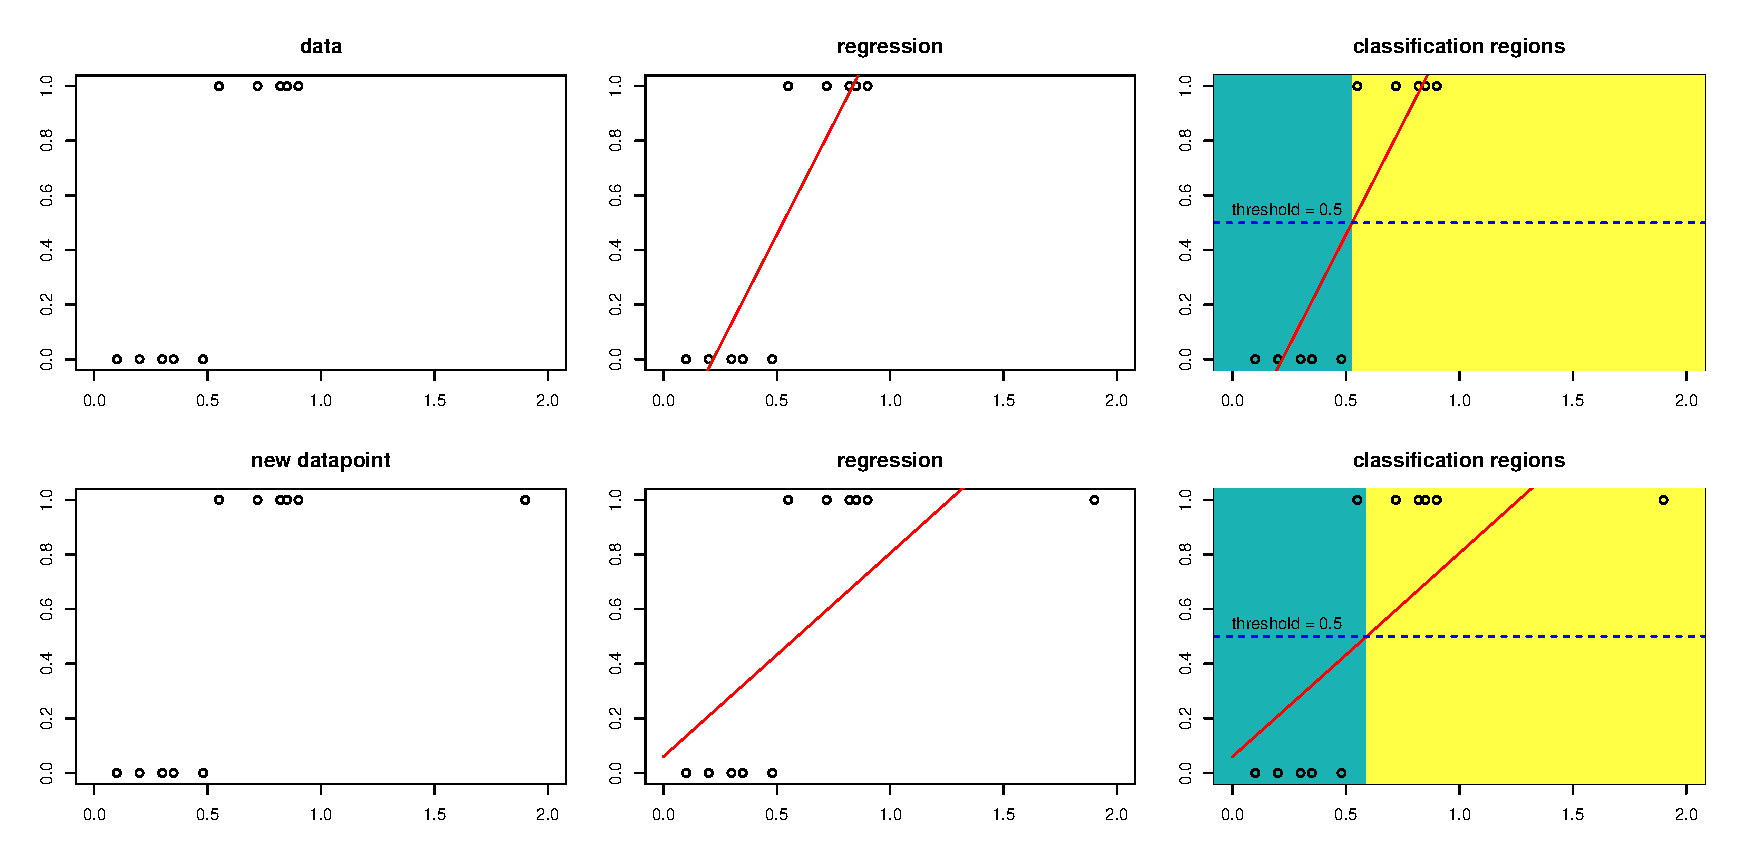
\includegraphics[width=5.5in]{03Linear/classRegressionThreshold.eps}
\end{center}
\caption{ตัวอย่างแสดงปัญหาการใช้การหาค่าถดถอยมาทำการจำแนกประเภท}
\label{fig: linear classification regression threshold}
\end{figure}
%

นอกจากปัญหาข้างต้นแล้ว ผลจากการหาค่าถดถอยยังอาจมีค่ามากกว่า $1$ มากๆ หรือน้อยกว่า $0$ มากๆ 
ซึ่งในการปฏิบัติแล้ว จะทำให้จัดการได้ยากมาก.
วิธีแก้ไขก็คือ แทนที่จะใช้การหาค่าถดถอยกับกลไกของ\textit{ขีดแบ่ง} ดังตัวอย่างข้างต้น 
เราจะใช้ตัวช่วยซึ่งได้แก่ \textit{โลจิสติกฟังชั่น} (Logistic Function หรือ อีกชื่อคือ\textit{ซิกมอยด์ฟังชั่น}, Sigmoid Function), \index{logistic function} \index{sigmoid function} \index{โลจิสติกฟังชั่น} \index{ซิกมอยด์ฟังชั่น}
\begin{eqnarray}
   h(a) = \frac{1}{1 + \exp (-a) }.
\label{eq: sigmoid function}
\end{eqnarray}

สำหรับงาน\textit{การจำแนกประเภทระหว่างสองกลุ่ม} (ฺBinary Classification) 
\index{binary classification} \index{การจำแนกประเภทระหว่างสองกลุ่ม} 
%, ที่แทนด้วย ค่า $0$ กับ $1$, 
เราสามารถทำนายค่ากลุ่ม $y \in \{0, 1\}$ จาก
\begin{eqnarray}
   y = h( f(\mathbf{x}, \mathbf{w}) )
\label{eq: logistic regression}
\end{eqnarray}
เมื่อ $h(\cdot)$ คือ\textit{โลจิสติกฟังชั่น} และ $f(x, \mathbf{w})$ คือฟังชั่นหาค่าถดถอย.
ฟังชั่นหาค่าถดถอยที่ง่ายที่สุดอันหนึ่ง คือ $f(\mathbf{x}, \mathbf{w}) = \mathbf{w}^T \cdot \mathbf{x}$.
วิธีนี้เรียกว่า \textit{โลจิสติกถดถอย} (Logistic Regression). 
\index{logistic regression} \index{โลจิสติกถดถอย}
รูป~\ref{fig: linear logistic} แสดงความสัมพันธ์ระหว่างอินพุตกับเอาต์พุตของโลจิสติกฟังชั่น.
สังเกตุ ค่าของเอาต์พุตจะอยู่ระหว่าง $0$ กับ $1$ โดยถ้าอินพุตมีค่ามากๆ ค่าเอาต์พุตจะใกล้กับ $1$.
ในขณะที่ถ้าอินพุตมีค่าน้อยๆ ค่าเอาต์พุตจะใกล้กับ $0$.

%
\begin{figure}
\begin{center}
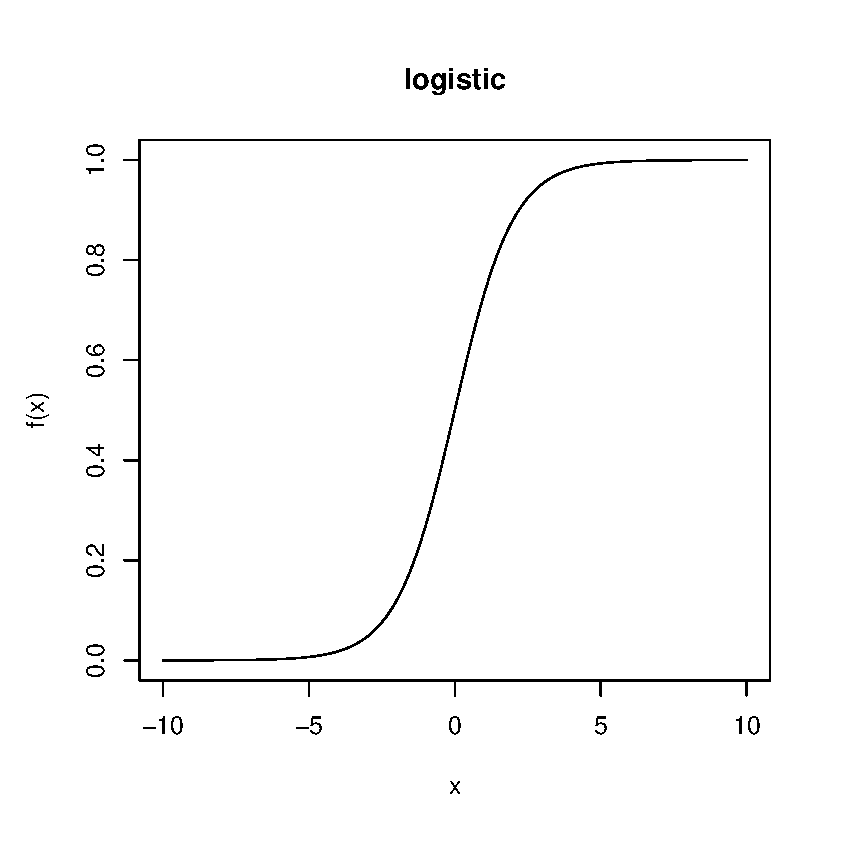
\includegraphics[height=2in]{03Linear/classLogistic.eps}
\end{center}
\caption{โลจิสติกฟังชัน}
\label{fig: linear logistic}
\end{figure}
%

\subsection{การฝึกโมเดลแบ่งกลุ่ม}
\label{sec: train binary classification}
\index{binary classification training}

\textit{วิธีโลจิสติกถดถอย}สามารถใช้ทำนายกลุ่มของข้อมูลได้แล้ว
เพียงแต่ก่อนจะใช้ โมเดลโลจิสติกถดถอยก็ต้องการค่าพารามิเตอร์ที่เหมาะสมเช่นกัน.
การฝึกโมเดลโลจิสติกถดถอยก็สามารถทำได้แบบเดียวกับการฝึกโมเดลการหาค่าถดถอย 
นั่นคือ หา $\mathbf{w}^* = \arg \min_{\mathbf{w}} E = \frac{1}{2} \sum_n \{ y(\mathbf{x}_n, \mathbf{w}) - t_n \}^2$, 
โดย $t_n \in \{0, 1\}$ คือ กลุ่มของจุดข้อมูลที่ $n$.
ฟังชั่นเป้าหมาย $E = \frac{1}{2} \sum_n \{ y(\mathbf{x}_n, \mathbf{w}) - t_n \}^2$ สามารถเรียกว่า \textit{ฟังชั่นค่าใช้จ่าย} (Cost Function)
\begin{eqnarray}
   \mathrm{Cost}( y(\mathbf{x}, \mathbf{w}), t) = \frac{1}{2} \{ y(\mathbf{x}, \mathbf{w}) - t\}^2.
\label{eq: linear cost function regression}
\end{eqnarray}

ดังนั้น การฝึกโมเดลสามารถเขียนในรูปของฟังชั่นค่าใช้จ่ายได้ ดังนี้
\begin{eqnarray}
   \mathbf{w}^* = \arg \min_{\mathbf{w}} \sum_n \mathrm{Cost}( y(\mathbf{x}_n, \mathbf{w}), t_n).
\label{eq: linear training}
\end{eqnarray}

สำหรับปัญหาการแบ่งกลุ่มสองกลุ่ม เนื่องจากค่า $t_n$ มีค่าเป็นไปได้แค่ $2$ ค่า 
ลักษณะพิเศษนี้สามารถนำมาใช้ประโยชน์เพื่อทำให้การฝึกโมเดลมีประสิทธิภาพมากขึ้นได้ 
โดยกำหนดให้
\begin{eqnarray}
   \mathrm{Cost}( y, t) = \left\{ \begin{array}{ll}
 -\log(y) & \quad \mbox{if} \quad t = 1, \\
 -\log(1-y) & \quad \text{if} \quad t = 0 \\
\end{array} \right.
\label{eq: linear cost function binary classification cases}
\end{eqnarray}
โดย เพื่อความกระทัดรัด บางครั้งจะเขียน $y$ แทน $y(\mathbf{x}, \mathbf{w})$.

สังเกตุ สมการ~\ref{eq: linear cost function binary classification cases},  
ค่าของ\textit{ฟังชั่นค่าใช้จ่าย}จะเป็น $0$ เมื่อ $t=1$ และ $y=1$ 
หรือ $t=0$ และ $y=0$. 
กล่าวง่ายๆคือ $\mathrm{Cost}( y, t) \to 0$ เมื่อโมเดลจำแนกประเภทได้ถูกต้อง.
%
ค่าของฟังชั่นจุดประสงค์จะเป็น $\infty$ เมื่อ $t = 1$ แต่ $y = 0$ 
หรือ เมื่อ $t = 0$ แต่ $y = 1$.
กล่าวง่ายๆคือ $\mathrm{Cost}( y, t) \to \infty$ เมื่อโมเดลจำแนกประเภทผิด.

จากสมการ~\ref{eq: linear cost function binary classification cases}, 
ฟังชั่นค่าใช้จ่ายสามารถเขียนในรูปที่กระชับขึ้นได้ ดังนี้
%
\begin{eqnarray}
   \mathrm{Cost}(y,t) = - t \cdot \log(y) - (1 - t) \cdot \log(1 - y).
\label{eq: linear cost function binary classification}
\end{eqnarray}

การฝึกโมเดล ซึ่งคือการแก้สมการ~\ref{eq: linear training} ต้องการเกรเดียนต์ของฟังชั่นค่าใช้จ่ายเทียบกับ $\mathbf{w}$.
เพื่อความกระทัดรัด กำหนดให้ $J \equiv \mathrm{Cost}$,
\begin{eqnarray}
   \nabla_{\mathbf{w}} J = \left[\frac{\partial J}{\partial w_0} \quad \frac{\partial J}{\partial w_1} \quad \frac{\partial J}{\partial w_2} \quad \cdots \quad \frac{\partial J}{\partial w_M}\right]^T
\label{eq: linear gradient cost function binary classification}
\end{eqnarray}
และ เมื่อแทนสมการ~\ref{eq: linear cost function binary classification} 
หาอนุพันธ์ ทำพีชคณิตและจัดรูป จนสุดท้ายจะได้ว่า
\begin{eqnarray}
   \frac{\partial J}{\partial w_m} &=& \left\{ y - t_n \right\} \cdot \phi_m(\mathbf{x}_n)
\label{eq: linear gradient J}
\end{eqnarray}
เมื่อ $y$ คือ ค่าที่ทำนายจากโมเดลโลจิสติกถดถอย $y(\mathbf{x}_n, \mathbf{w}) = h( \mathbf{w}^T \cdot \bm{\phi}(\mathbf{x}) )$,
ฟังชั่น $h(z)$ คือโลจิสติกฟังชั่น (สมการ~\ref{eq: sigmoid function},
และ $\bm{\phi}(\mathbf{x}) = 
[\phi_0(\mathbf{x}), 
\phi_1(\mathbf{x}),
\ldots ,
\phi_M(\mathbf{x})]^T$.

หากเลือกใช้ $\mathbf{\phi}(\mathbf{x}_n) = \mathbf{x}_n$, จะได้ว่า
\begin{eqnarray}
   \frac{\partial J}{\partial w_m} &=& \left\{ y(\mathbf{x}_n, \mathbf{w}) - t_n\right\} \cdot x_m^{(n)}
\label{eq: linear gradient logistic linear regression}
\end{eqnarray}
เมื่อ $x_m^{(n)}$ คือ ค่าอินพุตมิติที่ $m$ ของจุดข้อมูลที่ $n$ 
(กล่าวอีกอย่างคือ ค่าของฐานข้อมูลที่ เรคอร์ด $n$ ฟิลด์ที่ $m$).
ด้วยเกรเดียนต์ (สมการ~\ref{eq: linear gradient logistic linear regression}) วิธีลงเกรเดียนต์ก็สามารถนำมาใช้ในการฝึกโมเดลได้.

\subsection{ตัวอย่างการจำแนกประเภท}
\label{sec: logistic regression example}

กลับมาที่ตัวอย่างการจำแนกประเภท สำหรับปัญหาการทำนาย ผลตรวจโรคเบาหวานกับขนาดรอบเอว.
เมื่อใช้โมเดล\textit{โลจิสติกถดถอย} จะได้ผลดังแสดงในรูป~\ref{fig: linear classification log reg} 
ซึ่งจุดข้อมูลใหม่ไม่ได้ทำให้ผลการแบ่งกลุ่มเดิมที่ดีแล้วเปลี่ยนไป (เปรียบเทียบกับรูป~\ref{fig: linear classification regression threshold} ที่ใช้โมเดลการหาค่าถดถอย).
นอกจากนั้น เอาต์พุตจากโมเดลโลจิสติกถดถอยยังมีค่าอยู่ระหว่าง $0$ กับ $1$ 
ซึ่งสอดคล้องกับลักษณะงานมากกว่า และยังช่วยให้สามารถตีความในเชิงความน่าจะเป็นได้อีกด้วย.

กล่าวคือ เราอาจตีความได้ว่า เอาต์พุตจากโมเดล $y$ คือค่าทำนายความน่าจะเป็นที่จุดข้อมูลจะอยู่ในกลุ่ม $t = 1$ 
และเนื่องจากปัญหาการแบ่งกลุ่มนี้เป็นการแบ่งระหว่าง $2$ กลุ่ม 
ความน่าจะเป็นที่จุดข้อมูลน่าจะอยู่ในกลุ่มที่ $t = 0$ จะทำนายว่าประมาณ $1 - y$.
ดังนั้นหากความน่าจะเป็น $y$ มีค่ามากกว่า $0.5$ ก็ควรจะทายว่า จุดข้อมูลอยู่ในกลุ่ม $t = 1$.
ทำนองเดียวกัน ถ้า $y < 0.5$ (ความน่าจะเป็น $t=0$ คือ $1-y > 0.5$) ก็เหมาะสมที่จะทำนายว่า จุดข้อมูลอยู่ในกลุ่ม $t = 0$.

%
\begin{figure}
\begin{center}
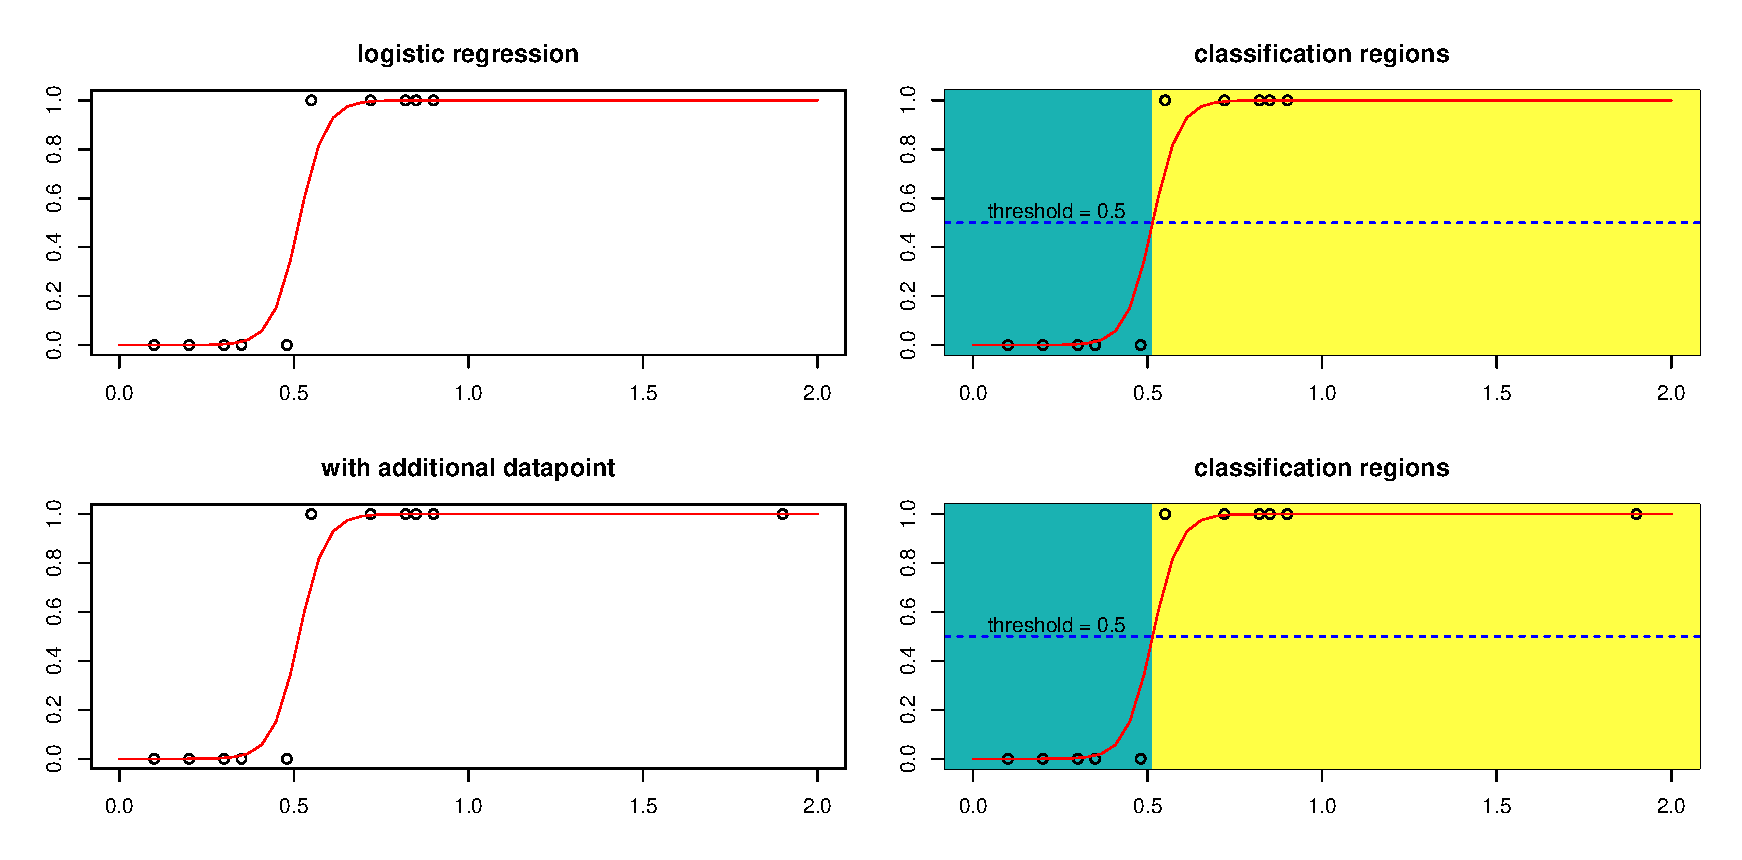
\includegraphics[height=2in]{03Linear/logregExample.eps}
\end{center}
\caption{ตัวอย่างการจำแนกประเภทด้วยวิธีโลจิสติกถดถอย 
เปรียบเทียบกับรูป~\ref{fig: linear classification regression threshold}.}
\label{fig: linear classification log reg}
\end{figure}
%

\paragraph{ตัวอย่างงานจำแนกกลุ่มข้อมูลชุดไอริส.}
ตัวอย่างปัญหาการจำแนกผู้ป่วยโรคเบาหวานจากขนาดรอบเอว แสดงปัญหาแบบที่อินพุตมีหนึ่งมิติ.
เพื่อให้เห็นภาพงานการจำแนกกลุ่มทั่วๆไปได้ดีขึ้น พิจารณาตัวอย่างปัญหาการจำแนกสปีชีส์ดอกไม้สกุลไอริสของ\textit{ข้อมูลชุดไอริส} (Iris Dataset\footnote{\textit{ชุดข้อมูลไอริส}จาก Edgar Anderson (1935) ซึ่งเป็นข้อมูลที่มาพร้อมกับ\textit{อาร์โปรเจค}
และสามารถเรียกใช้ได้ด้วยคำสั่ง \texttt{iris}, ดูคำอธิบายเพิ่มเติม \texttt{help(iris)}.})

{\small
\begin{shaded}
อนุกรมวิธาน (Taxonomy) คือวิธีการแบ่งกลุ่มของสิ่งมีชีวิตตามลักษณะร่วม.
เช่น โดเมน แบ่งตามลักษณะของเซลล์ ได้แก่ โพรแคริโอตที่เซลล์ไม่มีนิวเคลียส, 
อาร์เคียที่เซลล์ก็ไม่มีนิวเคลียส แต่มีเยื่อหุ้มเซลล์พิเศษที่ทำให้มันทดสภาพแวดล้อมที่รุนแรงได้,
และยูแคริโอตที่เซลล์มีนิวเคลียส.
หมายเหตุ ไวรัสนั้นไม่ครบเป็นเซลล์ในตัวเอง และไม่จัดอยู่ใน $3$ โดเมนนี้ 
แม้ความมีชีวิตของไวรัสเอง ก็ยังท้าทายนิยามของคำว่า``มีชีวิต''.

การจำแนกประเภทนี้ทำเป็นลักษณะของลำดับชั้น คือ โดเมน (Domain), อาณาจักร (Kingdom),
% มี 5 อาณาจักร: สัตว์, พืช, โพรทิสตา, ฟังไจ, มอเนอรา, และ อาจรวมถึง ไวรอยด์ สำหรับไวรัส ที่ ถ้าเป็นสิ่งมีชีวิต ก็เป็นชีวิตที่ไม่ครบเป็นเซลล์ในตัวเอง)
 ไฟลัม (Phylum) หรือ หมวด (Division) สำหรับอาณาจักรพืช, ชั้น (Class), อันดับ (Order) , วงศ์ (Family), สกุล (Genus), และ สปีชีส์ (Species) รวมถึงอาจมีหมวดหมู่แยกย่อยไปอีก เช่น ชนิดย่อย (subspecies).
มนุษย์จะถูกจัดอยู่ใน โดเมนยูแคริโอต, อาณาจักรสัตว์, ไฟลัมคอร์ดาตา (Chordata), ชั้นแมมอเลีย (Mammalia), อันดับไพรเมตส์ (Primates), วงศ์โฮมินิเดอิ (Hominidae), สกุลโฮโม (Homo), และ สปีชีส์โฮโมเซเปียน (Homo sapiens).
ขณะที่ลิงชิมแปนซี %ซึ่งเป็นญาติห่างๆของเรา 
ถูกจัดอยู่ โดเมน, อาณาจักร, ไฟลัม, ชั้น, อันดับ, และวงศ์ เดียวกับมนุษย์ แต่ ใช้ สกุลแพน (Pan) และสปีชีส์แพน โตรโกลไดเตส (Pan troglodytes).
\end{shaded}
}%

ข้อมูลชุดไอริสเก็บความยาวและความกว้างของกลีบดอกและกลีบเลี้ยงของดอกไม้สกุลไอริส $3$ สปีชี่ส์ที่มี 
\textit{ไอริส เซโทซา} (Iris setosa), 
\textit{ไอริส แวร์ซิคอเลอร์} (Iris versicolor), 
และ\textit{ไอริส เวอร์จินิกา} (Iris virginica).
หากต้องการจำแนกสปีชี่ส์ของดอกไม้สกุลไอริส จากความยาวและความกว้างของกลีบดอกและกลีบเลี้ยง
เนื่องจากกลุ่มสปีชี่ส์มี $3$ กลุ่ม
งานลักษณะนี้จะจัดเป็น งานการจำแนกกลุ่มแบบหลายกลุ่ม
ซึ่งจะอภิปรายต่อไปในหัวข้อ~\ref{section: multiclass classification}.
แต่เพื่อแนะนำแนวคิดของงานจำแนกกลุ่มเบื้องต้น ณ ที่นี้ จะอภิปรายการจำแนกกลุ่มระหว่างดอกที่เป็นสปีชี่ส์\textit{ไอริส เซโทซา}กับกลุ่มอื่นที่ไม่ใช่\textit{ไอริส เซโทซา}.

ถ้านำค่าความยาวของกลีบเลี้ยงและกลีบดอกจากชุดข้อมูลไอริสไปวาดจุดลงบนระนาบ
โดยให้แกนนอน (x-axis) แทนความยาวของกลีบเลี้ยง (sepal length) และแกนตั้ง (y-axis) แทนความยาวกลีบดอก (petal length) จะได้ภาพดังแสดงในภาพซ้ายบนในรูป~\ref{fig: linear classification decision boundary}.
%ของดอกไม้สกุลไอริสที่มี ไอริส เซโทซา (Iris setosa), ไอริส แวร์ซิคอเลอร์ (Iris versicolor), และไอริส เวอร์จินิกา (Iris virginica)  
%
รูป~\ref{fig: linear classification decision boundary} 
ภาพซ้ายบน
%แสดงจุดข้อมูลจากชุดข้อมูลไอริส.
จุดข้อมูลจากสปีชี่ส์\textit{ไอริส เซโทซา} (Iris setosa) เรียกเป็น กลุ่ม 1 แทนด้วยสัญญลักษณ์ `+'.
ส่วนจุดข้อมูลจากสปีชีส์อื่น ทั้ง\textit{ไอริส แวร์ซิคอเลอร์} (Iris versicolor) และ\textit{ไอริส เวอร์จินิกา} (Iris virginica) เรียกเป็น กลุ่ม 0 แทนด้วยสัญญลักษณ์ `x' ดังระบุในภาพ.

หลังจากนำข้อมูลไปฝึกโมเดลโลจิสติกถดถอย เราจะได้ค่าพารามิเตอร์ $\mathbf{w}$ ที่เหมาะสม
และเมื่อนำโมเดลโลจิสติกถดถอยที่ฝึกเสร็จแล้วไปทำนายผล ได้ผลดังแสดงในภาพบนขวา (รูป~\ref{fig: linear classification decision boundary}).
ผลการจำแนกกลุ่มด้วยโมเดลที่ฝึกมา
กลุ่ม 1 (\textit{ไอริส เซโทซา}) แสดงด้วยสัญญลักษณ์สี่เหลี่ยม
กลุ่ม 0 (\textit{ไอริส แวร์ซิคอเลอร์}หรือ\textit{ไอริส เวอร์จินิกา}) แสดงด้วยสัญญลักษณ์วงกลม.
สังเกตุ โมเดลสามารถจำแนกกลุ่มได้ถูกต้องทั้งหมด.

คุณสมบัติของโมเดลที่ได้ จะแบ่ง\textit{ปริภูมิอินพุต} (Input Space) 
ออกเป็นพื้นที่หรือย่านที่จะทายว่าเป็นกลุ่ม $1$ และย่านที่จะทายว่าเป็นกลุ่ม $0$ ดังแสดงในภาพล่างซ้ายมือ (รูป~\ref{fig: linear classification decision boundary}).
เนื่องจากเอาต์พุตของงานการจำแนกกลุ่มเป็นค่าไม่ต่อเนื่อง 
คุณสมบัติของโมเดลที่ใช้ในการแบ่งกลุ่มสามารถแสดงเป็นเขตบริเวณใน\textit{ปริภูมิอินพุต}ได้อย่างชัดเจน.

ย่านที่ทายกลุ่ม $1$ คือปริภูมิอินพุตบริเวณที่ทำให้ค่าเอาต์พุตของโลจิสติกถดถอย $y > 0.5$ 
เมื่อ $y = h( \mathbf{w}^T \mathbf{x} )$.
ซึ่งที่ $h( \mathbf{w}^T \mathbf{x} ) > 0.5$ ก็คือค่า $\mathbf{w}^T \mathbf{x} > 0$ (ดูรูป~\ref{fig: linear logistic} ประกอบ).
ทำนองเดียวกัน 
ย่านที่ทายกลุ่ม $0$ คือ $y < 0.5$ หรือ $\mathbf{w}^T \mathbf{x} < 0$.
ดังนั้น การใช้โมเดลในการจำแนกกลุ่ม จึงเสมือนเป็นการหาเส้นแบ่งเขตแดน ที่แบ่งระหว่างบริเวณของปริภูมิอินพุตที่จะทายว่าเป็นกลุ่ม $1$ กับบริเวณของกลุ่ม $0$
ซึ่งกรณีนี้ เส้นแบ่งนั้นอยู่ที่ $\mathbf{w}^T \mathbf{x} = 0$ ดังแสดงในภาพขวาล่างของรูป~\ref{fig: linear classification decision boundary}.
เส้นแบ่งนี้จะเรียกว่า \textit{เส้นแบ่งตัดสินใจ} (Decision Boundary).
\index{decision boundary}
\index{เส้นแบ่งตัดสินใจ}

%
%\begin{figure}
%\begin{center}
%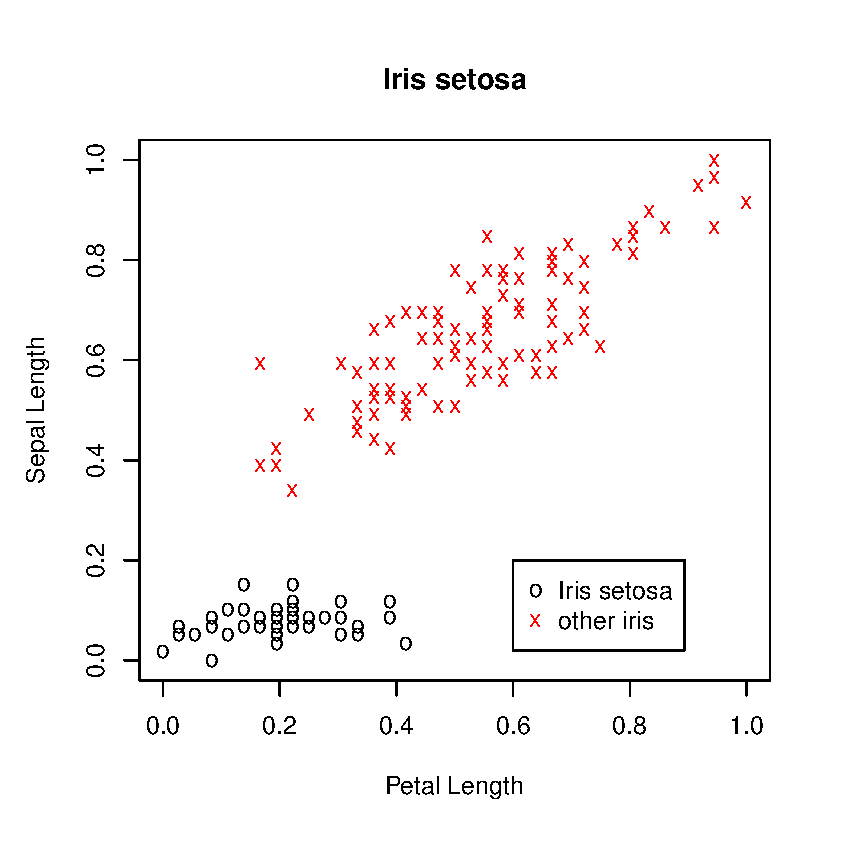
\includegraphics[height=3in]{03Linear/binaryExample.eps}
%\end{center}
%\caption{ตัวอย่างชุดข้อมูล Iris แสดงข้อมูลความยาวกลีบดอก (petal length) %กับกลีบเลี้ยง (sepal length) ของ Iris setosa และสปีชีส์อื่น.}
%\label{fig: linear binary classification iris}
%\end{figure}
%

% 
\begin{figure}
\begin{center}
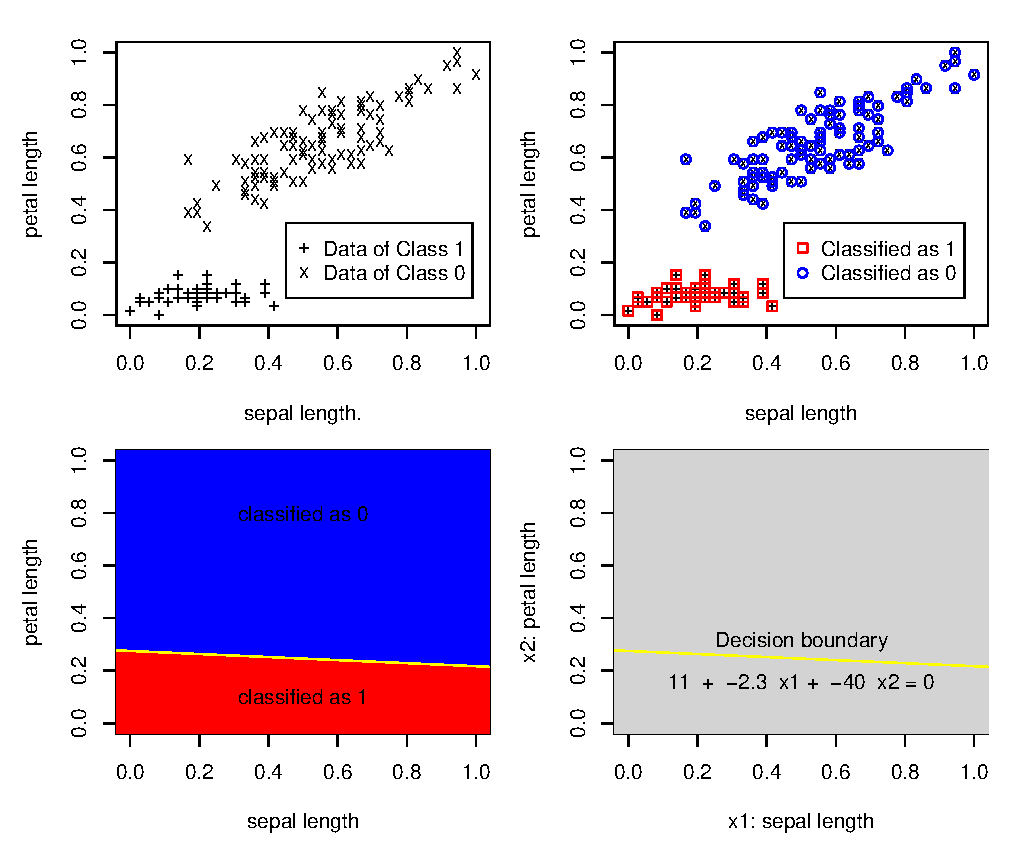
\includegraphics[width=5.5in]{03Linear/decisionBoundary.eps}
\end{center}
\caption{เส้นแบ่งตัดสินใจ.
ภาพซ้ายบน
แสดงจุดข้อมูลจากสปีชี่ส์\textit{ไอริส เซโทซา} (Iris setosa) เรียกเป็น กลุ่ม 1 แทนด้วยสัญญลักษณ์ `+'.
ส่วนจุดข้อมูลจากสปีชีส์อื่น ทั้ง\textit{ไอริส แวร์ซิคอเลอร์} (Iris versicolor) และ\textit{ไอริส เวอร์จินิกา} (Iris virginica) เรียกเป็น กลุ่ม 0 แทนด้วยสัญญลักษณ์ `x'.
%
ภาพขวาบน
แสดงผลการทำนายกลุ่มของแต่ละจุดข้อมูล
สัญญลักษณ์สี่เหลี่ยม แทนการทายเป็นกลุ่ม 1 (\textit{ไอริส เซโทซา})
สัญญลักษณ์วงกลม แทนการทายเป็นกลุ่ม 0 (\textit{ไอริส แวร์ซิคอเลอร์}หรือ\textit{ไอริส เวอร์จินิกา}).
%
ภาพซ้ายล่าง
แสดงบริเวณที่คุณสมบัติของโมเดลแบ่ง\textit{ปริภูมิอินพุต}
ออกเป็นบริเวณที่จะทายว่าเป็นกลุ่ม $1$ และบริเวณที่จะทายว่าเป็นกลุ่ม $0$.
%
ภาพขวาล่าง
แสดงเส้นแบ่งตัดสินใจระหว่างสองบริเวณ.
}
\label{fig: linear classification decision boundary}
\end{figure}
%

สำหรับโลจิสติกถดถอย ที่ใช้ $\mathbf{w}^T \mathbf{x}$ ซึ่งเป็นฟังชั่นเชิงเส้น จะทำให้ความสามารถในการจำแนกประเภทจำกัดอยู่เฉพาะกับข้อมูลที่สามารถแบ่งกลุ่มได้ดีด้วย\textit{เส้นแบ่งตัดสินใจ}ที่เป็นเส้นตรง (หรือ ระนาบสำหรับปริภูมิตอินพุตหลายๆมิติ) เท่านั้น 
และคุณภาพการแบ่งกลุ่มจะลดลง เมื่อใช้กับข้อมูลที่มีลักษณะดังแสดงในรูป~\ref{fig: linear classification nonlinear decision boundary}.
ซึ่งปัญหานี้อาจแก้ได้โดยใช้เบซิสฟังชั่นที่มีลักษณะ\textit{ไม่เป็นเชิงเส้น} (non-linear) 
เช่น การใช้ดีกรีที่สูงขึ้น  ได้แก่แทนที่จะใช้ $y = h( w_0 + w_1 x_1 + w_2 x_2)$ 
อาจจะใช้ $y = h( w_0 + w_1 x_1 + w_2 x_1^2 + w_3 x_2 + w4 x^2 + w5 x_1 x_2)$ หรือ ดีกรีที่สูงขึ้นตามจำเป็น.
แต่วิธีนี้นอกจากการจะไม่สะดวกแล้ว ยังทำได้ยากในทางปฏิบัติกับข้อมูลที่มีมิติสูงๆ 
ซึ่งสำหรับข้อมูลมิติสูงๆแล้ว การตรวจสอบดูความสัมพันธ์ระหว่างอินพุตจะทำได้ยาก.
บทที่~\ref{chapter: ANN} และ~\ref{chapter: others} อภิปรายถึงโมเดลที่มีประสิทธิภาพในการสร้าง\textit{เส้นแบ่งตัดสินใจที่มีลักษณะไม่เป็นเชิงเส้น} (Non-Linear Decision Boundary).

% 
\begin{figure}
\begin{center}
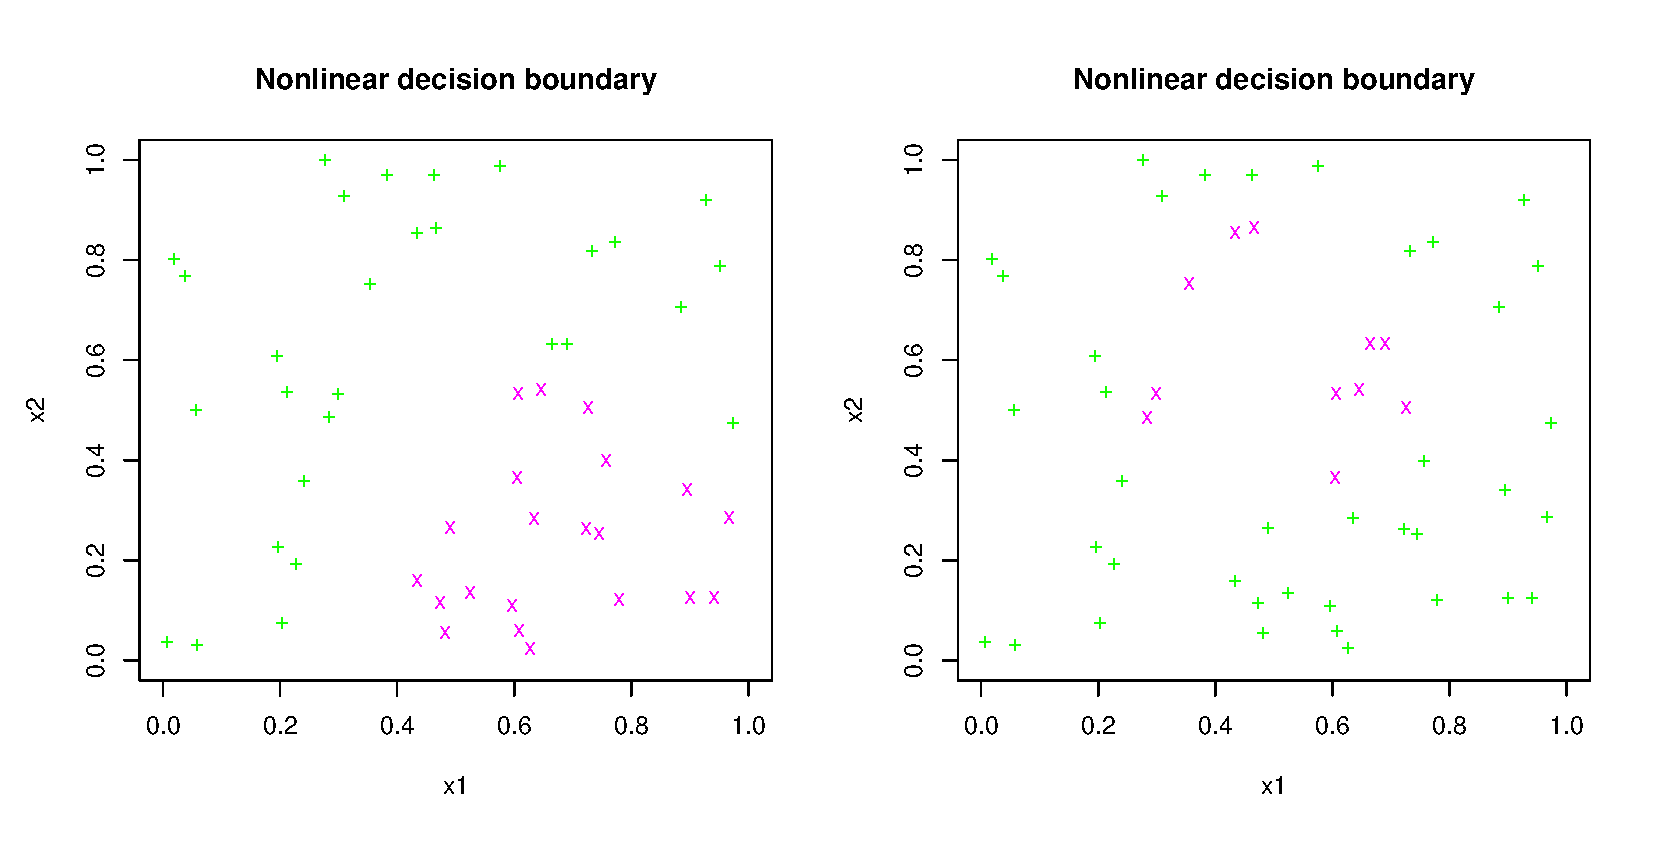
\includegraphics[width=5.5in]{03Linear/nonlinDecisionBoundary.eps}
\end{center}
\caption{ตัวอย่างแสดงชุดข้อมูลที่ต้องการเส้นแบ่งตัดสินใจที่มีลักษณะไม่เป็นเชิงเส้น.
สัญญลักษณ์ `+' แทนจุดข้อมูลของกลุ่ม 1
สัญญลักษณ์ `x' แทนจุดข้อมูลของกลุ่ม 0.
ภาพซ้าย กรณีที่ต้องการเส้นแบ่งตัดสินใจในลักษณะเส้นโค้ง.
ภาพขวา กรณีที่ต้องการเส้นแบ่งตัดสินใจในลักษณะเส้นวงกลม}
\label{fig: linear classification nonlinear decision boundary}
\end{figure}
%

\subsection{การจำแนกประเภทแบบหลายกลุ่ม}
\label{section: multiclass classification}
\index{multiclass classification}
\index{การจำแนกประเภทแบบหลายกลุ่ม}

ตัวอย่างที่อภิปรายข้างต้นเป็นการจำแนกประเภทแบบ $2$ กลุ่ม.
ถ้าหากต้องการ\textit{จำแนกประเภทแบบหลายกลุ่ม} (Multiclass Classification) 
\index{multiclass classification}
ก็สามารถทำได้ง่ายๆคือ แทนที่จะใช้เอาต์พุต $1$ มิติ ($t \in \{0, 1\}$ เราจะใช้เอาต์พุต $K$ มิติ 
โดยให้ $K$ เท่ากับจำนวนกลุ่ม
และจะสร้างโมเดลที่ทำให้สำหรับแต่ละอินพุต จะมีเอาต์พุตแค่มิติเดียวเท่านั้นที่มีค่าเป็น $1$ ที่เหลือจะมีค่าเป็น $0$
ซึ่งการจัดการลักษณะนี้จะเรียกว่า \textit{การเข้ารหัสหนึ่งไปเค} (1-of-K Coding), 
$\mathbf{t} \in \{0,1\}^K$  และ $\sum_{k=1}^K t_k = 1$.

ฟังชั่นค่าใช้จ่ายอาจจะถูกนิยามในลักษณะเดียวกับสมการ~\ref{eq: linear cost function binary classification},
%
\begin{eqnarray}
\mathrm{Cost}(\mathbf{y}, \mathbf{t}) = -\sum_{k=1}^K \left\{ t_k \ln y_k + (1-t_k) \ln (1 - y_k) \right\}.
\label{eq: linear cost function multiclass complement}
\end{eqnarray}
%
สมการ~\ref{eq: linear cost function multiclass complement} อาจตีความได้ว่า 
คือ \textit{ลบลอการิทึ่มของค่าความควรจะเป็น} โดย\textit{ความควรจะเป็นของกลุ่ม}ที่อินพุต $\mathbf{x}$ และโมเดล $\mathbf{y}(\mathbf{x}, \mathbf{w})$ คือ
%
\begin{eqnarray}
   p(\mathbf{t}|\mathbf{x}, \mathbf{w}) = \prod_{k=1}^K y_k (\mathbf{x}, \mathbf{w})^{t_k} \cdot \left( 1 - y_k(\mathbf{x}, \mathbf{w}) \right)^{1-t_k}.
\label{eq: linear likelihood function multiclass complement}
\end{eqnarray}

ตัวอย่าง \textit{ชุดข้อมูลไอริส}ที่มีจุดข้อมูลของความยาวและความกว้างของกลีบดอก (petal) และกลีบเลี้ยง (sepal) ดอกไม้ในสกุลไอรีส อยู่ $3$ สปีชีส์
\textit{ไอริส เซโทซา} (Iris setosa), 
\textit{ไอริส แวร์ซิคอเลอร์} (Iris versicolor), 
และ\textit{ไอริส เวอร์จินิกา} (Iris virginica).
ภาพตัวอย่างของดอกไม้ในสกุลไอรีส แสดงในรูป~\ref{fig: linear Iris flowers}.

% 
\begin{figure}
\begin{center}
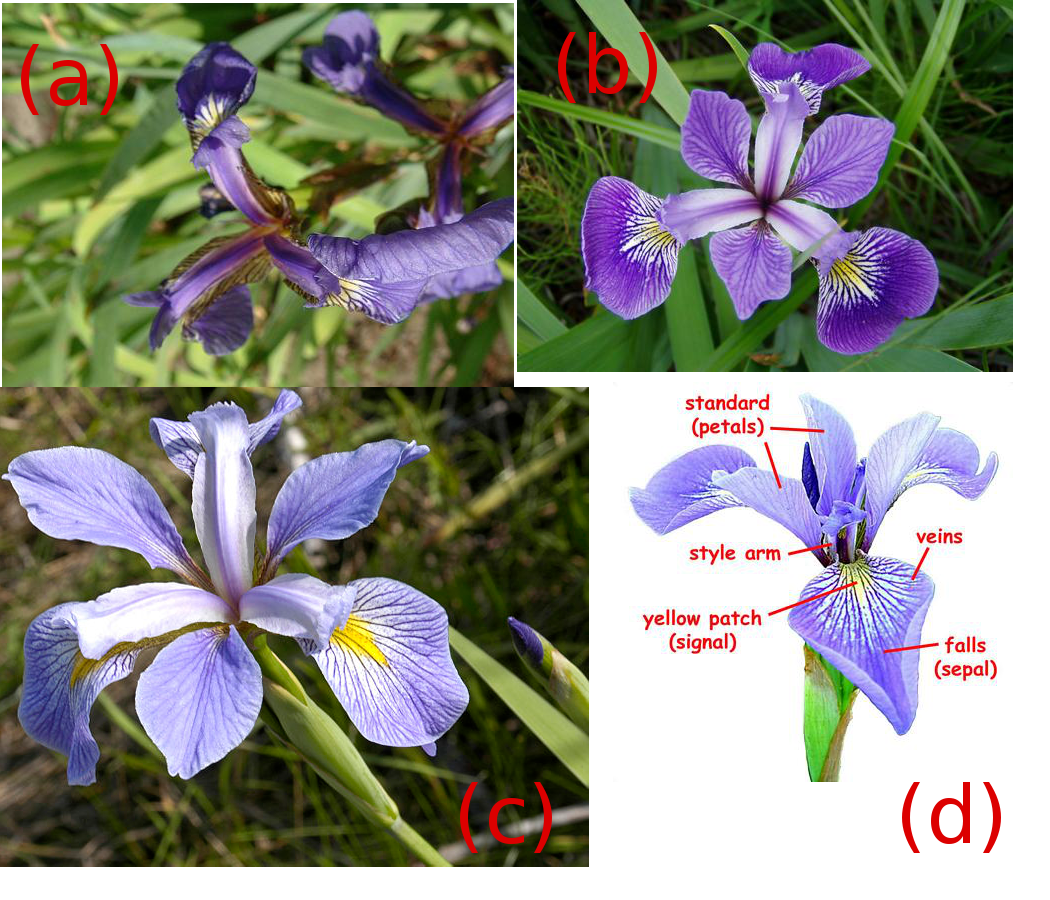
\includegraphics[width=5.5in]{03Linear/IrisPicsPNG.png}
\end{center}
\caption{ตัวอย่างของดอกไม้ในสกุลไอรีส.
ภาพ a ตัวอย่างดอก\textit{ไอริส เซโทซา}.
ภาพ b ตัวอย่างดอก\textit{ไอริส แวร์ซิคอเลอร์}.
ภาพ c ตัวอย่างดอก\textit{ไอริส เวอร์จินิกา}.
ภาพ d แสดงส่วนประกอบของดอก รวมถึงกลีบดอกและกลีบเลี้ยง.
{\footnotesize ภาพ a-c จาก Wikimedia Commons: Radomil Binek (29 May 2005, \url{http://en.wikipedia.org/wiki/File:Kosaciec_szczecinkowaty_Iris_setosa.jpg}), Danielle Langlois (July 2005, \url{http://en.wikipedia.org/wiki/File:Iris_versicolor_3.jpg}), Frank Mayfield (28 May 2007, \url{http://en.wikipedia.org/wiki/File:Iris_virginica.jpg}).
ภาพ d จาก \url{http://www.fs.fed.us/wildflowers/beauty/iris/flowers.shtml}, วันที่ดึงข้อมูล 25 ม.ค. พ.ศ.2557)} }
\label{fig: linear Iris flowers}
\end{figure}
%

ข้อมูลชุดนี้มี $150$ จุดข้อมูล 
แต่ละจุดข้อมูลมีค่า\textit{คุณลักษณะ} (attributes) อยู่ $4$ ค่า
ได้แก่ ความยาวกลีบเลี้ยง (Sepal Length), 
ความกว้างกลีบเลี้ยง (Sepal Width), 
ความยาวกลีบดอก (Petal Length) 
และความกว้าง (Petal Width).
และมีเฉลยเอาต์พุตหรือฉลากบอกสปีชี่ส์.
ข้อมูลชุดนี้มีฉลากอยู่ $3$ กลุ่ม \texttt{setosa}, \texttt{versicolor}, และ \texttt{virginica}.
\textit{คุณลักษณะ}ทั้ง $4$ จะใช้เป็นอินพุต ($\mathbf{x} \in \mathbb{R}^4$) 
และฉลากบอกสปีชี่ส์เป็นเอาต์พุต 
โดยให้เอาต์พุตเป็น 
$t = [1 \quad 0 \quad 0]^T$ แทนจุดข้อมูลที่เป็น \texttt{setosa}, 
$t = [0 \quad 1 \quad 0]^T$ แทนจุดข้อมูลที่เป็น \texttt{versicolor}, 
และ $t = [0 \quad 0 \quad 1]^T$ แทนจุดข้อมูลที่เป็น \texttt{virginica}.

BREAK HERE

รูป~\ref{fig: linear classification iris boxplot} แสดงช่วงของค่าอินพุตที่มิติต่างๆของจุดข้อมูลทั้ง $3$ กลุ่ม โดย
กลุ่ม 1 แทน \texttt{setosa}, 
กลุ่ม 2 แทน \texttt{versicolor}, 
และกลุ่ม 3 แทน \texttt{virginica}.
สังเกตุว่าการแบ่งข้อมูลชุดนี้ จะไม่ยากนัก เนื่องจากแม้ว่าอินพุตจะเป็น $4$ มิติ แต่ค่า \texttt{Petal.Length} หรือ \texttt{Petal.Width} ของจุดข้อมูลจากกลุ่มต่างๆ แยกตัวกันดีพอสมควร.
โดยเฉพาะการแยกกลุ่ม 1 นั้นสามารถใช้ค่าของ \texttt{Petal.Length} หรือ \texttt{Petal.Width} ก็สามารถจำแนกจุดข้อมูลกลุ่ม 1 ออกจาก $2$ กลุ่มที่เหลือได้อย่างถูกต้องแล้ว.
รูป~\ref{fig: linear classification iris 2D projections} แสดงจุดข้อมูล (ที่อยู่ในปริภูมิ $4$ มิติ) เมื่อนำมาวาดลงบนระนาบ $2$ มิติด้วยอินพุตคู่ต่างๆ.
เห็นได้ชัดว่าเราสามารถใช้ระนาบเส้นตรงแยกกลุ่ม โดยเฉพาะกลุ่ม 1 ออกมาได้.
%
แต่อย่างไรก็ตาม %เราเพียงใช้ข้อมูลชุดนี้ เพื่อเป็นตัวอย่างการจำแนกประเภทแบบหลายกลุ่ม ดังนั้นเรา
ตัวอย่างนี้จะใช้อินพุตทั้ง $4$ มิติในการสร้างโมเดลเพื่อจำแนกประเภท.

% 
\begin{figure}
\begin{center}
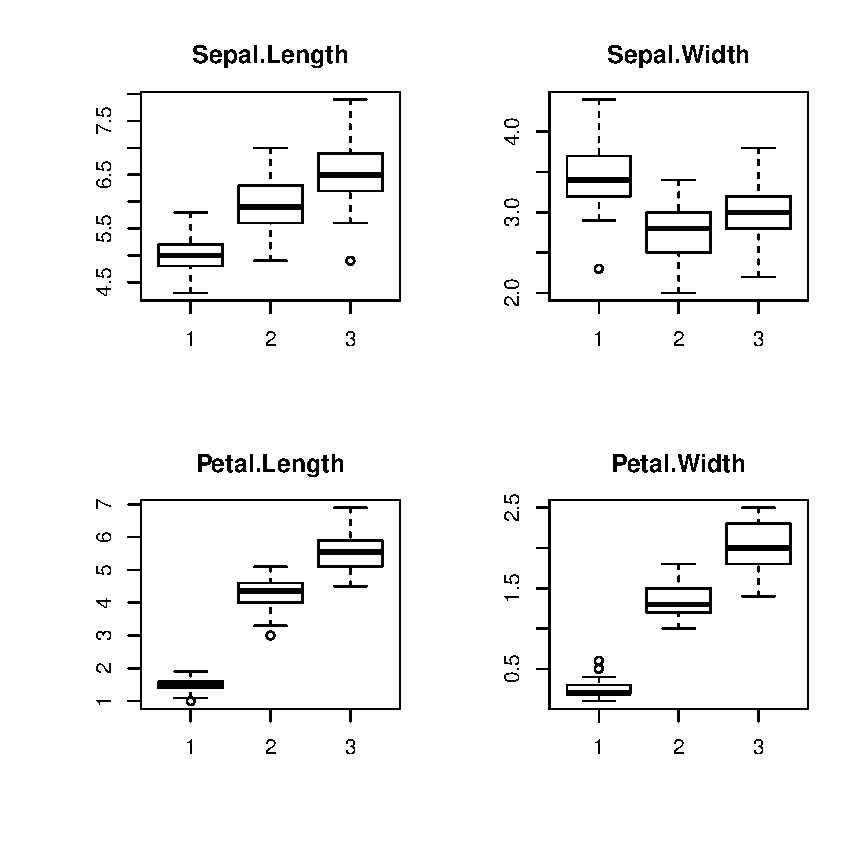
\includegraphics[width=5.5in]{03Linear/irisBoxplot.eps}
\end{center}
\caption{แสดงช่วงของค่าอินพุตมิติต่างๆ 
โดยกลุ่ม 1 แทน \texttt{setosa}, 
กลุ่ม 2 แทน \texttt{versicolor}, 
และกลุ่ม 3 แทน \texttt{virginica}.}
\label{fig: linear classification iris boxplot}
\end{figure}
%

% 
\begin{figure}
\begin{center}
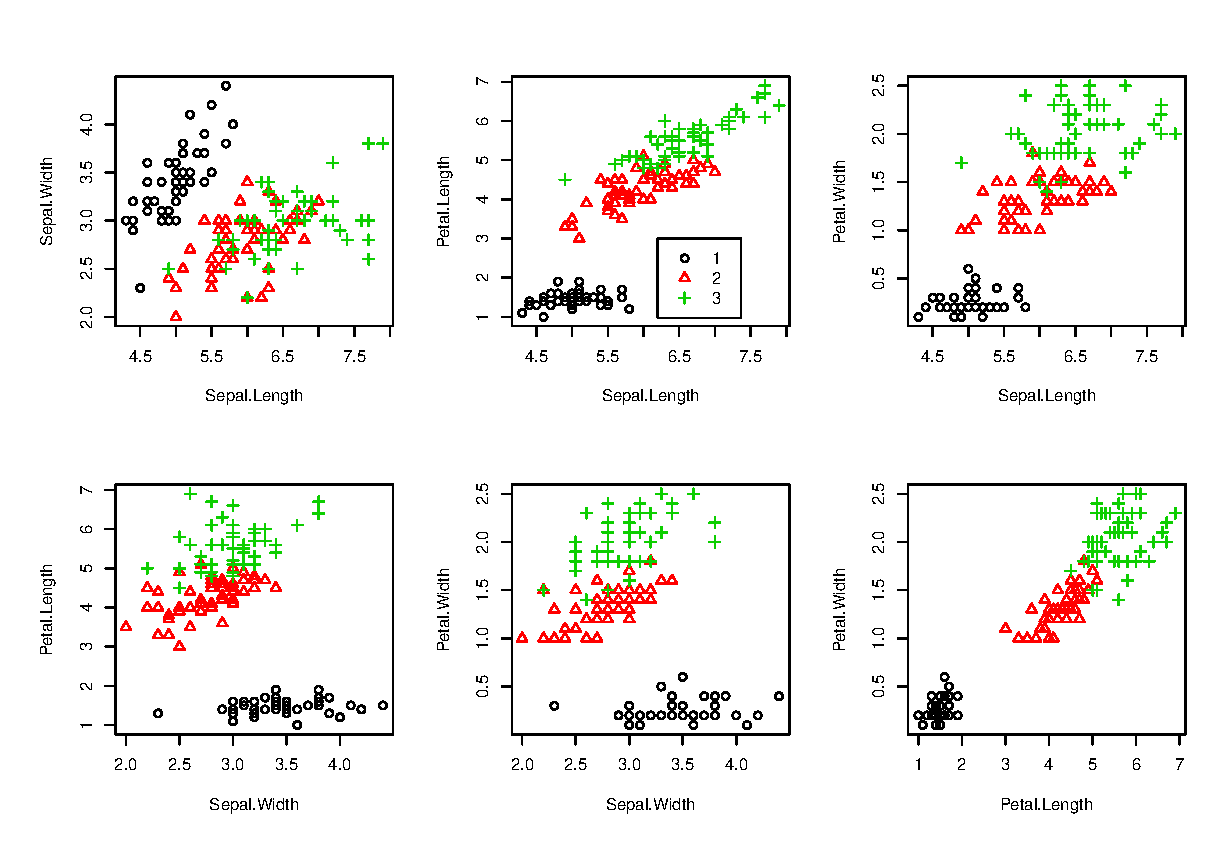
\includegraphics[width=5.5in]{03Linear/iris6plots.eps}
\end{center}
\caption{จุดข้อมูลเมื่อวาดลงบนระนาบ $2$ มิติ ด้วยค่าอินพุตคู่ต่างๆ}
\label{fig: linear classification iris 2D projections}
\end{figure}
%

เริ่มด้วยการฝึกโมเดล เพื่อหาค่า $\mathbf{w}^* =\arg \min_{\mathbf{w}} \sum_{n=1}^N \mathrm{Cost}(\mathbf{y}(\mathbf{x}_n, \mathbf{w}), \mathbf{t}_n)$. (ดูแบบฝึกหัดท้ายบทข้อ 6)
สมมติค่าพารามิเตอร์ที่ได้ $\mathbf{w}^*$ คือ
\begin{verbatim}
> W
          [,1]       [,2]       [,3]
[1,]  1.154165  1.0913158 -0.4060659
[2,]  0.829558  0.4565969 -2.1633640
[3,]  3.432528 -1.6508103 -1.5221858
[4,] -5.667041  0.5354391  2.9062448
[5,] -1.735660 -1.3257176  2.4796421
\end{verbatim}
สำหรับ $3$ กลุ่ม (ตามคอลัมน์ สำหรับกลุ่ม 1 กลุ่ม 2 และกลุ่ม 3 %setosa, versicolor, virginica 
ตามลำดับ) และ $5$ คุณลักษณะ ได้แก่ $[1, x_1, x_2, x_3, x_4]^T$ (ตามแถว สำหรับ\textit{ไบอัส} 
(bias), \texttt{Sepal.Length}, \texttt{Sepal.Width}, \texttt{Petal.Length},
และ \texttt{Petal.Width} ตามลำดับ).

หลังจากได้ค่าพารามิเตอร์ $\mathbf{w}^*$ แล้ว 
นำค่าที่ได้มาใช้ร่วมกับโมเดลเพื่อทำนายกลุ่ม เช่น 
การจำแนกประเภทด้วยโลจิสติกถดถอยกับลักษณะเชิงเส้น
\[
\mathbf{y} = [h(\mathbf{w}_1^T \mathbf{x}), \; h(\mathbf{w}_2^T \mathbf{x}), \; h(\mathbf{w}_3^T \mathbf{x})]^T
\]
โดย จากตัวอย่างข้างต้น,
\[ 
\mathbf{w}_1 = [1.154165,\; 0.829558,\; 3.432528,\; -5.667041,\; -1.735660]^T
\]
เป็นต้น.
ดังนั้นเมื่อนำมาคำนวณกับค่า $\mathbf{x}$ เช่น ถ้าจุดข้อมูลมีค่า
\begin{verbatim}
Sepal.Length  Sepal.Width Petal.Length  Petal.Width 
         5.1          3.5          1.4          0.2 
\end{verbatim}
จะได้ $\mathbf{x} = [1, \; 5.1, \; 3.5, \; 1.4, \; 0.2]$, 
และคำนวณได้ว่า
$y_1 = h( \mathbf{w_1}^T \mathbf{x} ) = h( 9.117769 ) = 0.9998903$
เช่นเดียวกัน 
จะได้ว่า $y_2 = 0.1331482$ 
และ $y_3 = 5.019370 \times 10^{-6}$ 
หรือกล่าวง่ายๆ คือ
\[
\mathbf{y} = [0.9998903,\; 0.1331482,\; 5.019370 \times 10^{-6}]^T.
\]

เมื่อเปรียบเทียบค่าทั้งสามแล้วพบว่า $y_1$ มีค่ามากที่สุด ดังนั้นจะทายว่า จุดข้อมูลจุดนี้น่าจะอยู่ กลุ่มที่ 1.
รูป~\ref{fig: linear classification iris classified datapoints} แสดงตัวอย่างผลจากการทำนายกลุ่มด้วยโมเดล.
จะเห็นว่าส่วนใหญ่โมเดลทำนายได้อย่างถูกต้อง ซึ่งเมื่อคิดเป็นตัวเลขรวม คือ ทายถูก $96.7 \%$\footnote{การประเมินผล โมเดลที่ถูกต้องจะต้องทำการทดสอบกับข้อมูลที่ไม่ได้ถูกใช้ในการฝึกโมเดล (ดูหัวข้อ~\ref{section: Model selection}) แต่ผลที่แสดงในหัวข้อนี้ มีจุดประสงค์เพื่อประกอบคำอธิบายเรื่องวิธีการจำแนกประเภท และไม่ได้ทดสอบกับข้อมูลอีกชุด.}.
%
ตาราง~\ref{tbl: linear iris classification results} แจกแจงผลการจำแนกประเภทแต่ละกลุ่ม
ด้วย\textit{เมตริกซ์สับสน} (Confusion Matrix).
จะเห็นว่า โมเดลสามารถจำแนกจุดข้อมูลจากกลุ่ม 1 ได้ถูกต้องสมบูรณ์ 
ในขณะที่ยังสับสนกับข้อมูลจากกลุ่ม 2 และ 3 บ้าง.
นั่นคือ มีจุดข้อมูลจริงอยู่กลุ่มที่ 2 แล้วทายผิดว่าเป็นกลุ่ม 3 อยู่ที่ $8\%$.
การแจกแจงเช่นนี้จะช่วยให้เข้าใจความเสี่ยงของการใช้โมเดลได้ดีขึ้น 
โดยเฉพาะการนำไปใช้งานกับข้อมูลที่ละเอียดอ่อน เช่น แอพพลิเคชั่นด้านการแพทย์ เป็นต้น.

% 
\begin{figure}
\begin{center}
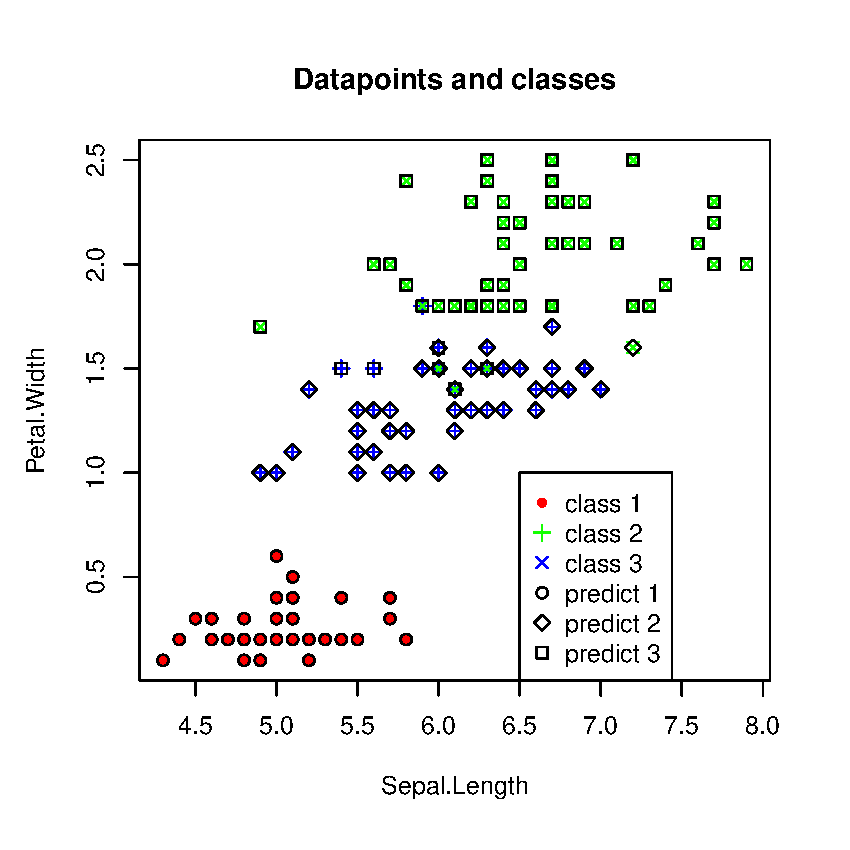
\includegraphics[width=5.5in]{03Linear/irisMulticlass.eps}
\end{center}
\caption{แสดงจุดข้อมูลของชุดข้อมูลไอริสบนระนาบ $2$ มิติ
โดย แกนนอนแทน \texttt{Sepal.Length} 
และแกนตั้งแทน \texttt{Petal.Width}.
กลุ่มจริง 1 ถึง 3 (\texttt{class 1-3}) และกลุ่มที่ทำนาย (\texttt{predict 1-3}) 
ใช้สัญญลักษณ์ตามระบุในภาพ.
หมายเหตุ การทำนายใช้ข้อมูลครบทั้ง $4$ มิติ แต่เพื่อความสะดวกจึงเลือกแสดงบนระนาบ $2$ มิติ}
\label{fig: linear classification iris classified datapoints}
\end{figure}
%
\begin{table}[hbtp]
\caption{เมตริกซ์สับสน. ผลการจำแนกประเภทชุดข้อมูลไอริสสำหรับแต่ละกลุ่ม}
\begin{center}
\begin{tabular}{|r|c|c|c|}
\hline 
กลุ่มจริง & ทายเป็นกลุ่ม 1 & ทายเป็นกลุ่ม 2 & ทายเป็นกลุ่ม 3 \\
\hline
1 & 100$\%$ & 0$\%$ & 0$\%$ \\
\hline
2 & 0$\%$ & 92$\%$ & 8$\%$ \\
\hline
3 & 0$\%$ & 2 $\%$ & 98$\%$ \\ 
\hline
\end{tabular} 
\end{center}
\label{tbl: linear iris classification results}
\end{table}

\section{แบบฝึกหัด}
\label{section: linear exercises}

%\subsection{regression}

\paragraph{1.} จงเขียนโปรแกรมเพื่อนำสมการ~\ref{eq: linear W} และ~\ref{eq: linear beta} ไปปฏิบัติ
และสาธิตการใช้งาน.

\paragraph{2.} จงเขียนโปรแกรมเพื่อนำสมการ~\ref{eq: linear w online linear model} ไปปฏิบัติ
สาธิตการใช้งาน และเปรียบเทียบกับแบบฝึกหัดข้อ 1.

\paragraph{3.} จงแสดงในเห็นว่าค่า $\mathbf{w}$ ในสมการ~\ref{eq: linear w regularization} จะทำให้ค่าผิดพลาดรวม (สมการ~\ref{eq: linear total error function}) มีค่าน้อยที่สุด.

%\subsection{logistic regression}

\paragraph{4.} จากตัวอย่างปัญหาการจำแนกกลุ่มของคนเป็นโรคเบาหวานจากขนาดรอบเอว 
โดยมีข้อมูล ดังแสดงในตาราง~\ref{tbl: linear ex logistic regression diabetes}, 
\texttt{N} แทน\textit{ผลลบ} และ \texttt{P} แทน\textit{ผลบวก}.
จงทดลองใช้โมเดลโลจิสติกถดถอยในการจำแนกกลุ่ม 
และทดลองทำอีกครั้งเมื่อมีข้อมูลเพิ่ม คือ $(x,y) = (1.90, P)$.
เปรียบเทียบผลที่ได้กับรูป~\ref{fig: linear classification log reg}.

{\small
\begin{table}[hbtp]
\caption{ข้อมูลปัญหาขนาดรอบเอวกับผลตรวจโรคเบาหวาน.
x แทนค่านอร์มอไลซ์ของขนาดรอบเอว
และ y แทนผลการตรวจเบาหวาน}
\begin{center}
\begin{tabular}{|r|c|c|c|c|c|c|c|c|c|c|}
\hline 
%ค่านอร์มอไลซ์ของขนาดรอบเอว 
x & 0.10 & 0.21 & 0.31 & 0.35 & 0.48 & 0.55 & 0.85 & 0.72 & 0.82 & 0.90 \\
\hline
%ผลการตรวจเบาหวาน  
y &   N &   N &   N &    N &    N &    P &    P &      P    &    P &   P \\
\hline
\end{tabular} 
\end{center}
\label{tbl: linear ex logistic regression diabetes}
\end{table}
}

\paragraph{5.} จงหาอนุพันธ์ของฟังชั่นต่อไปนี้
\begin{itemize}
\item $f(x) = 1/\left\{ 1 + \exp(-x) \right\}$ และแสดงให้เห็นว่า $f'(x) = \{1 - f(x)\} \cdot f(x)$.
\item $f(x,y) = x \cdot \log( y )$ เทียบกับ $y$.
\item แสดงว่าเกรเดียนต์ของสมการ~\ref{eq: linear cost function binary classification} เทียบกับ $w_m$ คือ สมการ~\ref{eq: linear gradient J}.
\end{itemize}
คำใบ้
\begin{itemize}
\item $\frac{d \log(x)}{d x} = \frac{1}{x}$.
\item ถ้า $y$ เป็นฟังชั่นของ $x$ และ $f$ เป็นฟังชั่นของ $y$, 
แล้วจากกฏลูกโซ่ (Chain Rule) ได้ว่า
$\frac{d f}{d x} = \frac{d f}{d y} \cdot \frac{d y}{d x}$.
\end{itemize}

\paragraph{6.} สำหรับฟังชั่นลักษณะใดๆ $\phi_m(\mathbf{x})$, เช่น $\phi_m(\mathbf{x}) = x_m$ สำหรับลักษณะเชิงเส้นดีกรีหนึ่ง 
หรือ $\phi_m(\mathbf{x}) = \exp( - \frac{(\mathbf{x} -\mathbf{\mu}_m )^2}{\sigma_m} ) $ สำหรับลักษณะแบบเกาส์เชี่ยน, จงหาอนุพันธ์,
\[
\frac{\partial \mathrm{C}}{\partial w_{mk}} 
=\frac{\partial \sum_{n=1}^N \mathrm{C}_n}{\partial w_{mk}}
\]
เมื่อ $\mathrm{C}_n \equiv \mathrm{Cost}(\mathbf{y}(\mathbf{x}_n, \mathbf{w}), \mathbf{t}_n)$ นิยามดังสมการ~\ref{eq: linear cost function multiclass complement} 
และ $\mathbf{y} = [y_1 \; y_2 \; \cdots \; y_K]^T$ โดย
$y_k = h( \mathbf{w}_k^T \mathbf{\phi}) = 1/(1 + \exp( \mathbf{w}_k^T \mathbf{\phi}))$;
$\mathbf{\phi} = [\phi_0(\mathbf{x}) \; \phi_1(\mathbf{x}) \; \cdots \; \phi_M(\mathbf{x})]^T$;
$\mathbf{w}_k = [w_{0k} \; w_{1k} \; \cdots \; w_{Mk}]^T$
แล้ว จงแสดงให้เห็นว่า
\begin{eqnarray}
   \frac{\partial C}{\partial w_{km}} &=& -\sum_{n=1}^N \left\{ \frac{t_{nk}}{y_{nk}} - \frac{(1 - t_{nk})}{(1 - y_{nk})} \right\} \cdot \frac{\partial y_{nk}}{\partial w_{km}}
\nonumber \\
   &=& -\sum_{n=1}^N \left\{ t_{nk} (1-y_{nk}) - (1-t_{nk}) y_{nk} \right\} \cdot \phi_m(\mathbf{x}_n)
\nonumber \\   
   &=& -\sum_{n=1}^N \left\{ y_{nk} - t_{nk} \right\} \cdot \phi_m(\mathbf{x}_n)
\label{eq: linear multicass grad dual cost}
\end{eqnarray}
เมื่อ
\[
   \frac{\partial y_{nk}}{\partial w_{km}} = \left\{ 1 - h(\mathbf{w}_k^T \mathbf{\phi}) \right\} \cdot h(\mathbf{w}_k^T \mathbf{\phi}) \cdot \phi_m(\mathbf{x}_n).
\]

\paragraph{7.} จงเขียนโปรแกรมเพื่อสร้างโมเดลจำแนกประเภทชุดข้อมูลไอรีส โดยใช้โมเดลโลจิสติกถดถอยกับ โมเดลเชิงเส้นดีกรีหนึ่ง $\phi_m(\mathbf{x}) = x_m$
และทดสอบโมเดลที่ได้กับชุดข้อมูลไอรีส เปรียบเทียบกับผลที่แสดงในหัวข้อ~\ref{section: multiclass classification}.

\paragraph{8.} จงแบ่งข้อมูลเป็นชุดฝึกหัดและชุดทดสอบก่อน แล้วจงใช้วิธีโลจิสติกถดถอยกับโมเดลเชิงเส้นดีกรีหนึ่ง ในการจำแนกประเภท พร้อมประเมินประสิทธิภาพของโมเดล.

\paragraph{9.} จงใช้โลจิสติกถดถอยกับโมเดลเชิงเส้นดีกรีหนึ่ง ในการจำแนกประเภทของชุดข้อมูลไวน์ โดยประเมินผลการทำงานด้วยวิธีครอสวาลิเดชั่น (ดูหัวข้อ~ \ref{section: Model selection})